%%%%%%%%%%%%%%%%%%%%%%%%%%%%%%%%%%%%%%%%%%%%%%%%%%%%%%%%%%%%%%%%%%% 
%                                                                 %
%                            CHAPTER                              %
%                                                                 %
%%%%%%%%%%%%%%%%%%%%%%%%%%%%%%%%%%%%%%%%%%%%%%%%%%%%%%%%%%%%%%%%%%% 
 
\chapter{Implementation}


\section{Camera setup}
Tests of the setup: 

\begin{itemize}
\item 3D printing the tool holder
\item 3D printing a easy way of photographing many tools in an easy way
\end{itemize}




Parts of the setup:

\begin{enumerate}
\item leds
	\begin{enumerate}
	\item 3-4 led lights/strips separately controllable to light from different angles
	\item with or without extra light on top
	\end{enumerate}
\item Wheel with tool mount
	\begin{enumerate}
	\item 3D model creation of mount system
	\item creating wheel to be accurate
	\item controlling stepper motor to turn just enough to put the next tool in front of the camera
	\end{enumerate}
\item Camera mount
	\begin{enumerate}
	\item Design to let the camera view different angles
	\item watch out for lighting
	\end{enumerate}
\end{enumerate}

Also a pcb 

\section{Designing a tool holder}
During the design process different tool holders are designed to create an optimel camera position and optimal lighting conditions for that setup.
\subsection{Simple tool holder}
test remote second
\subsection{Wheel holder}
First Wheel Holder:

A simple wheel holder which can hold 20 inserts.

used for first tests and did work. Except the tools wern't fixed good enough or they were to hard to remove and insert into the holder.

The holder was printed badly and this made the print cleanup very labor intensive. 

Second Wheel Holder:

Created on the base of the first wheel holder, but with an easier way of inserting and removing the tools. 

This with a more secure way of holding the tools. 

print so no cleanup must be done

\subsubsection{first wheel holder}

Created vrijdag 13 november 2020



To be able to quickly create a lot of photos in a consistant way, a wheel is designed to mount 20 tools at once; using a stepper motor and a fixed camera and lighting setup the process of taking images would be automated for every 20 tools. The holder will be 3D printed so a few wheels can be made to be able to swap the wheels with new tools for an efficient dataset creation.



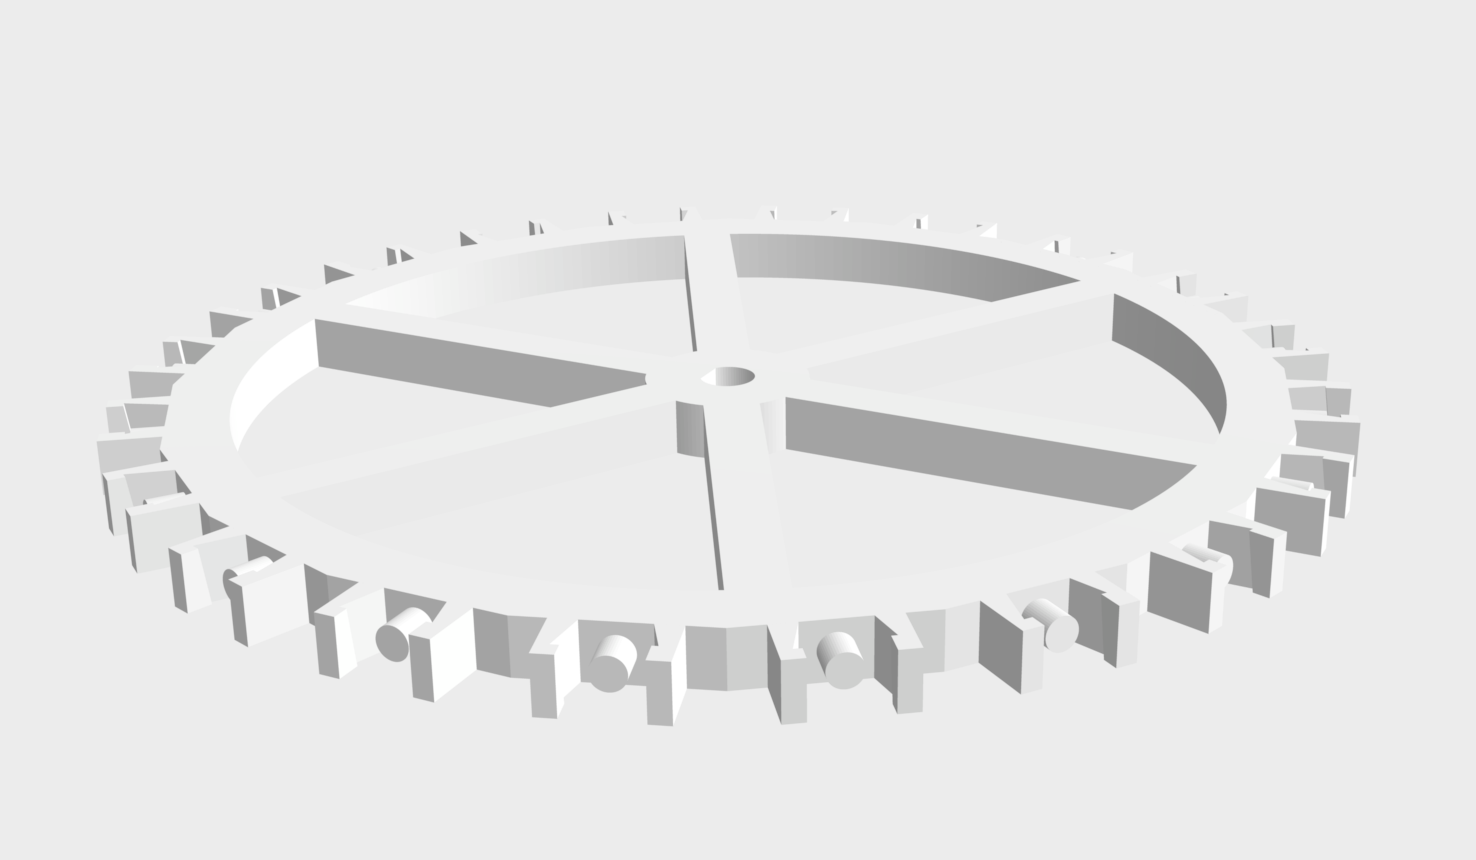
\includegraphics[height=3.125000in, keepaspectratio=true]{./fig/Camera_setup/Tool_Holder/Wheel_Holder/first_wheel_holder/radhouder.png}



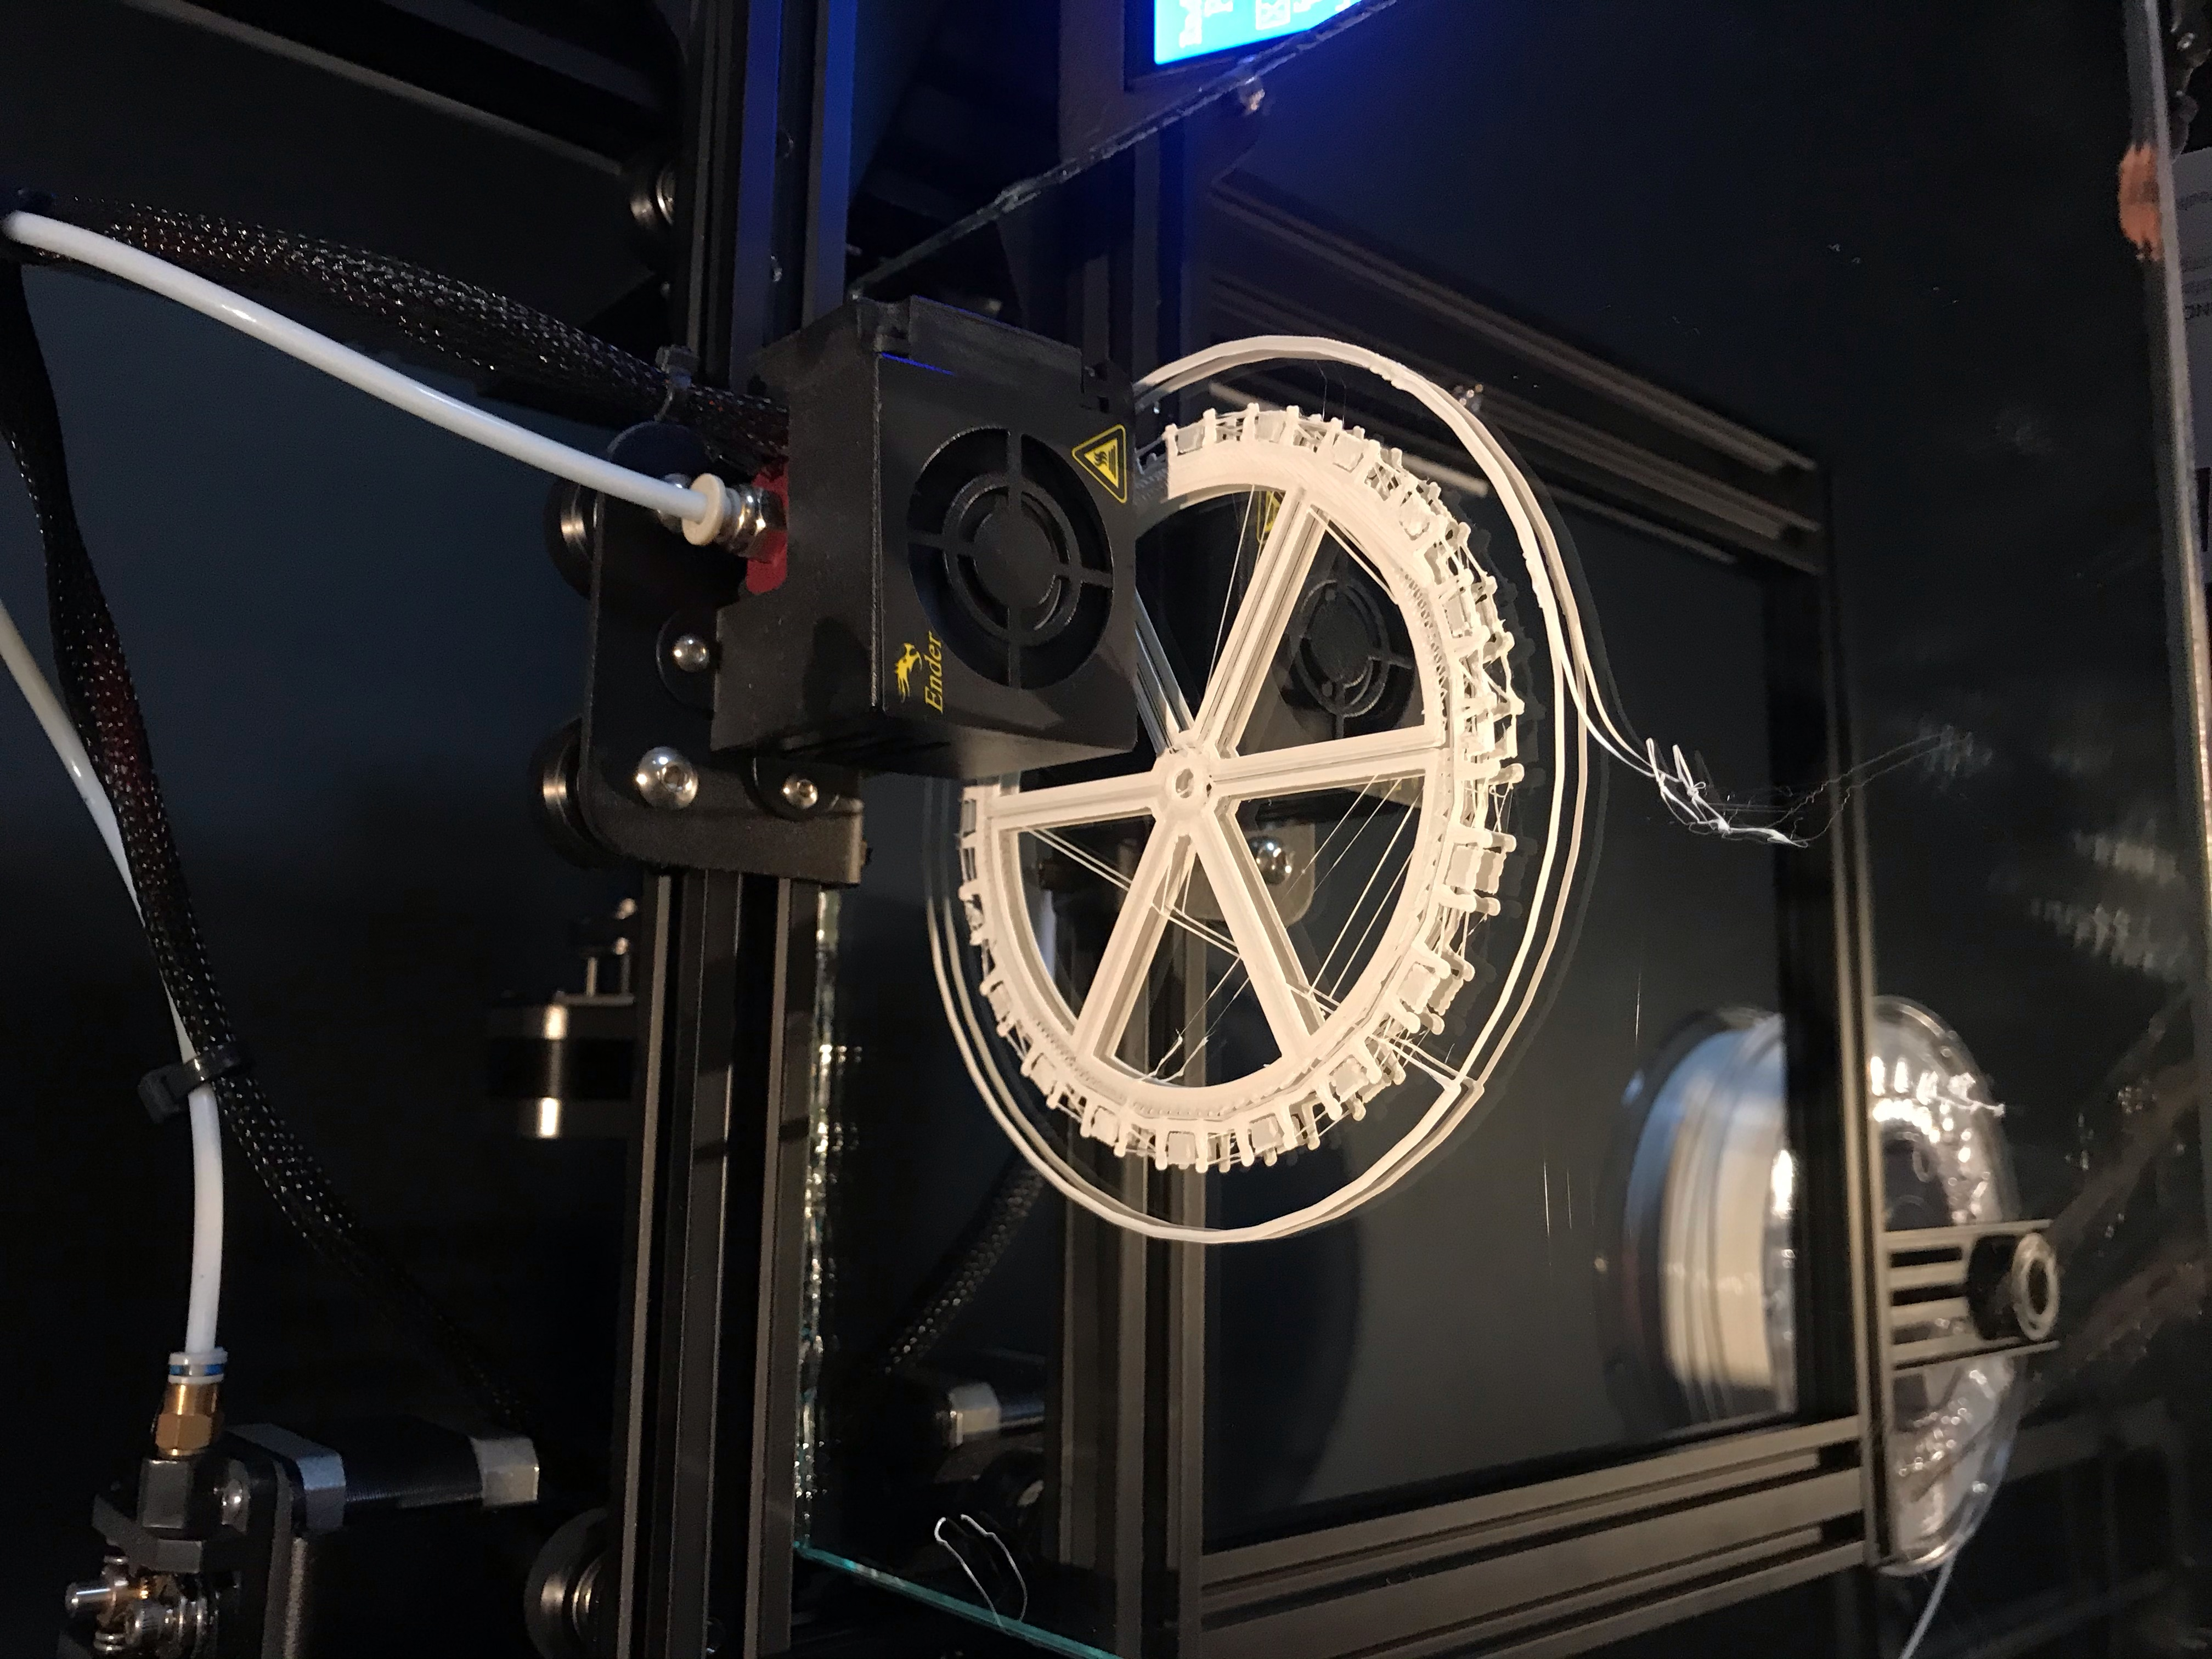
\includegraphics[height=3.125000in, keepaspectratio=true]{./fig/Camera_setup/Tool_Holder/Wheel_Holder/first_wheel_holder/radhouder_duringprint.jpeg}

After printing the wheel had to be cleared from rest pieces of plastic and had to be tested with a tool, this made it possible to scratch the tool extra hard which would mean the given labels for that tool aren't correct anymore. The tool used is from 3 number 6 36*. the manual removal also means the tools dont sit in the same position in every place on the wheel. This will show in the generated pictures.

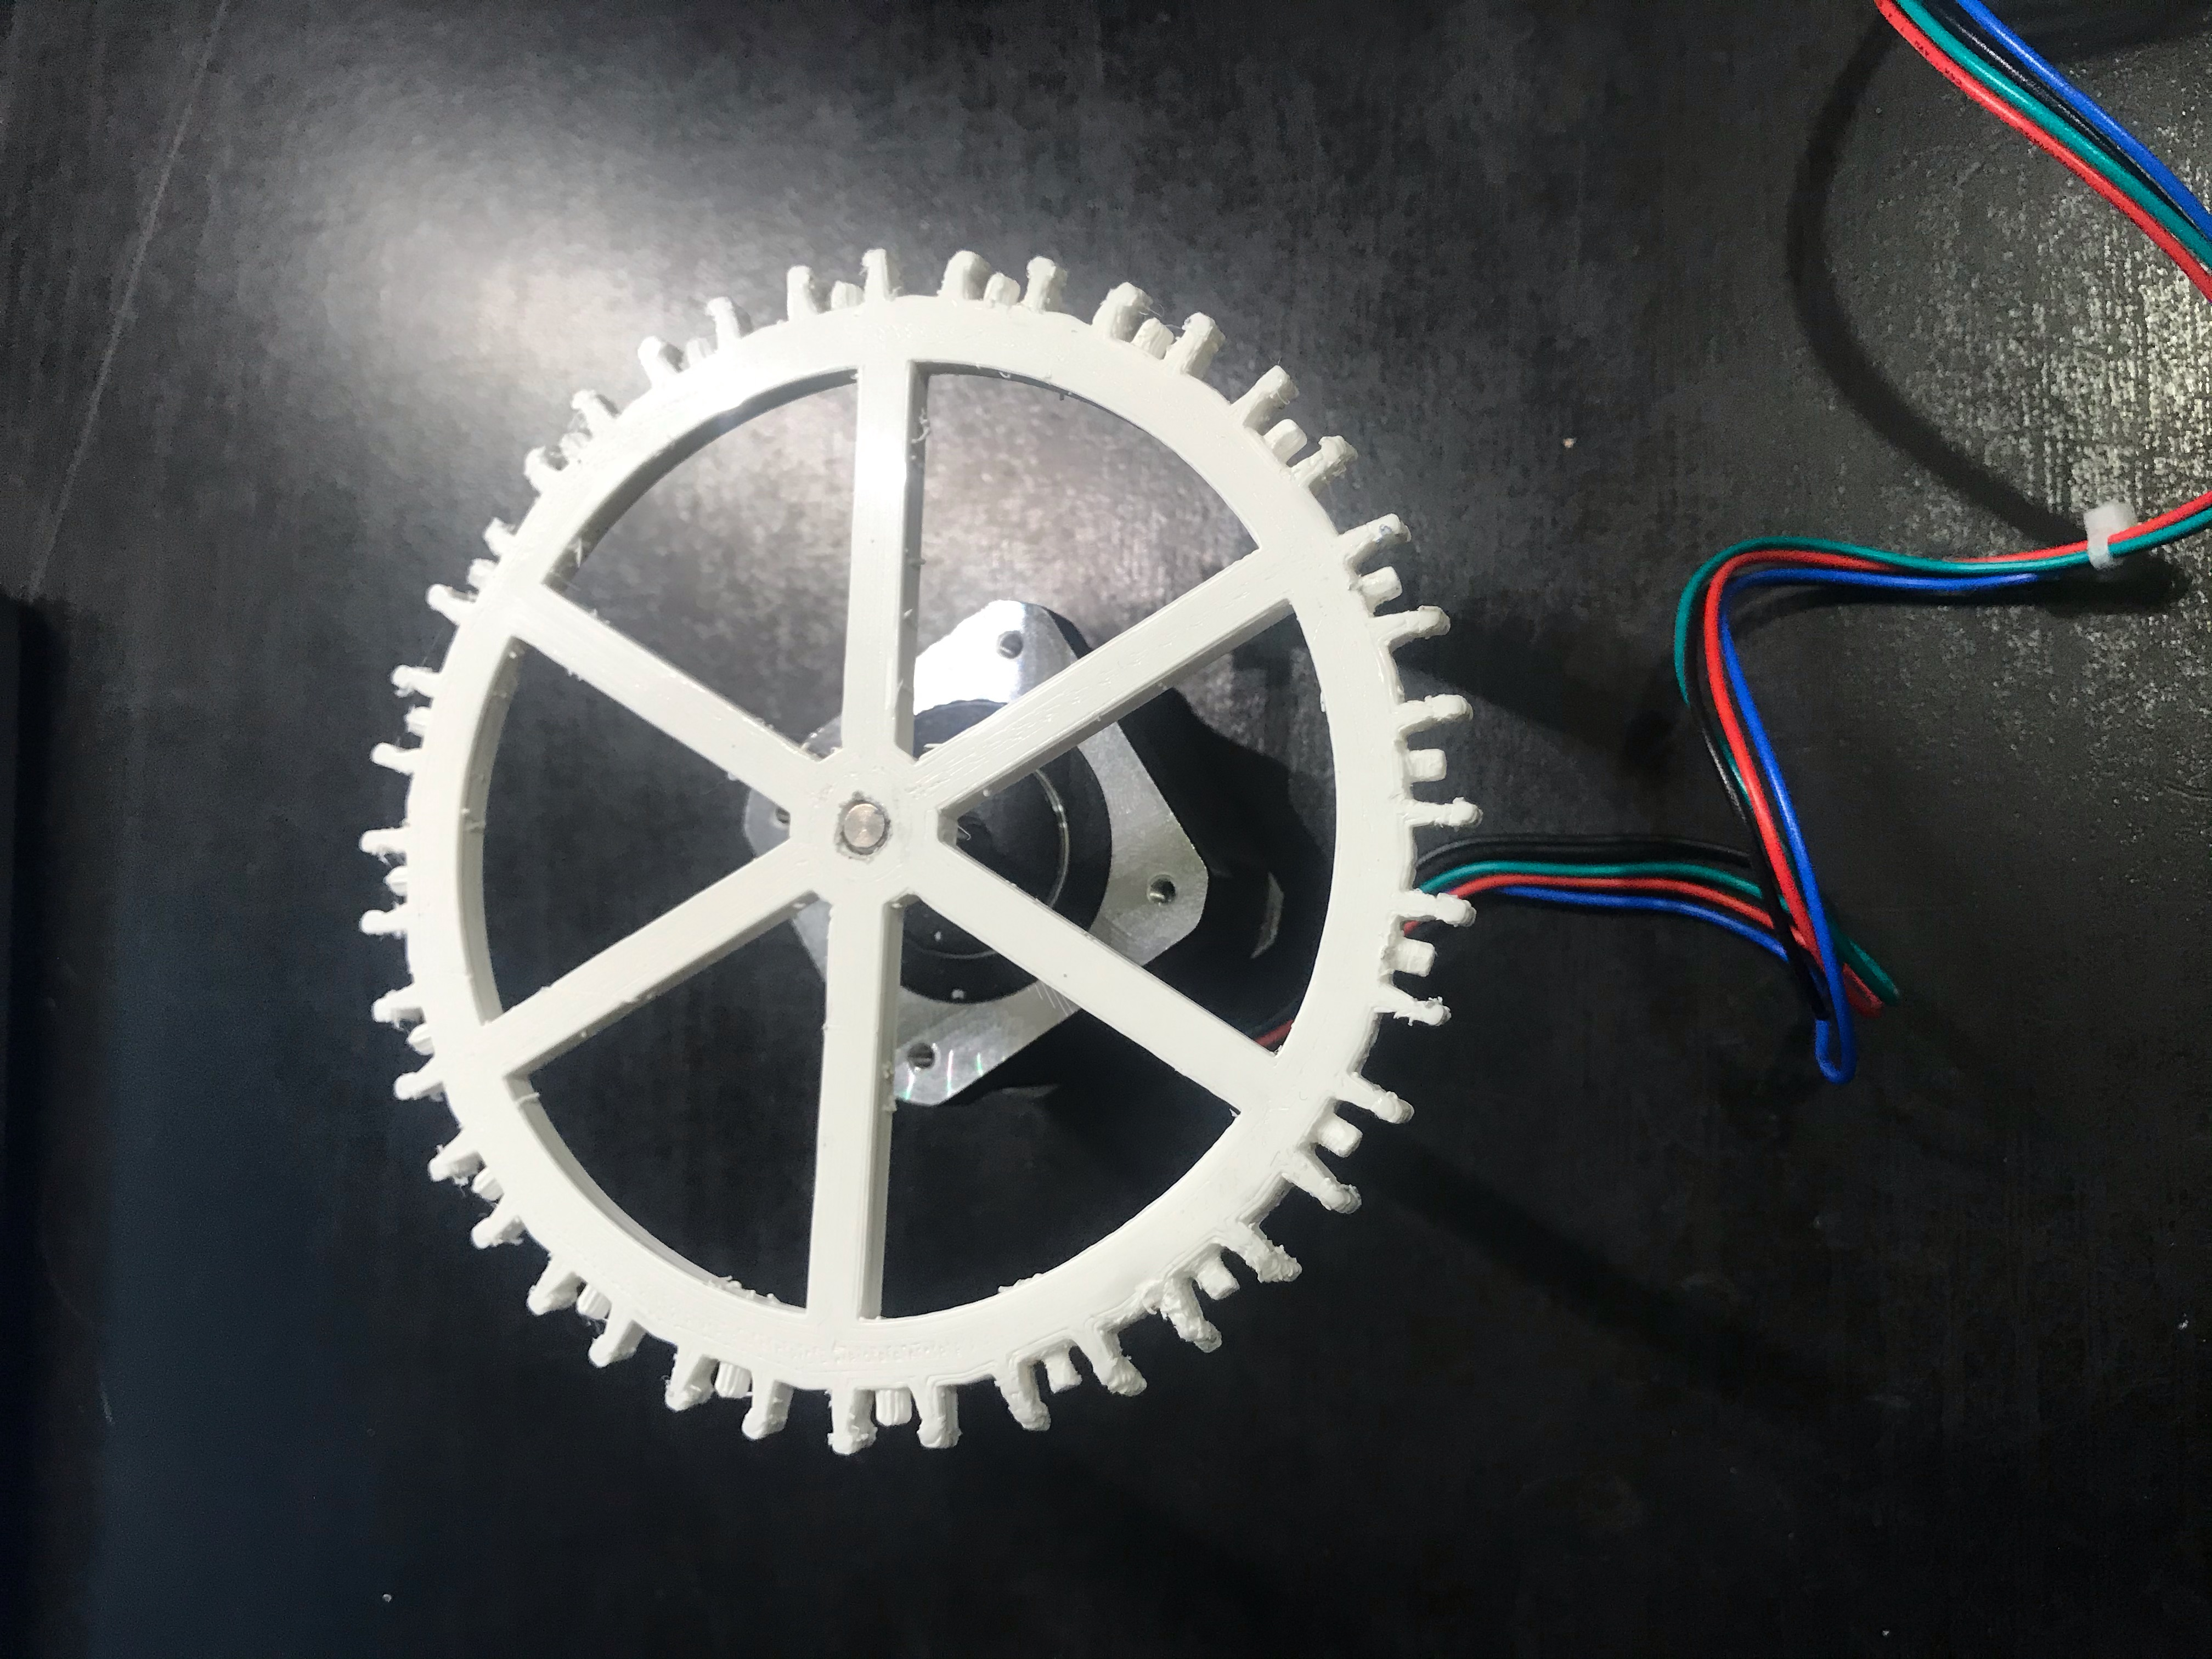
\includegraphics[height=3.125000in, keepaspectratio=true]{./fig/Camera_setup/Tool_Holder/Wheel_Holder/first_wheel_holder/radhouder_horizontal.jpeg}



This wheel is mounted on a stepper motor with step angle of 1.8 degrees.

We can calculate the accuracy for a wheel with a radius of 5.5cm (measured to the tip of the measured tool) 

grad to radials

2*pi/360*1.8= 0.0314159265359

sin(0.031415)*55 = 1.72754081497 mm



this gives an accuracy of 1.72 mm, this is not in the accuracy range that is needed for this project. In order to get the wanted displacement per step the rotations needs to be adjusted with extra gears in the system. A displacement of less than 0.5 mm would be good.



to achieve this the calculations are made backworth:

the required angle

arcsin(0.5/55) = 0.52 degrees 

calculate how the gears should relate to each other

1.8/0.52 = 3.46153846154



round this up to 4 and recalculate the displacement per step of the motor

the angle:

1.8/4 = 0.45

2*pi/360*0.45= 0.00785398163397

sin(0.00785398163397)*55 = 0.431964548879mm



This is whithin the needed displacement range.



This needs adjustment of the current design of the wheel holder also a 3d printed footer can be printed so the wheel can circulate vertically which would make the camera and light setup easier.

\subsubsection{Second Wheel Holder}

Created vrijdag 04 december 2020



The first wheel holder wasn't good because the inserts where clamped in with the knife side so it was very hard to remove them.

In a new wheel holder the clamps got changed by new clips that can easily be removed and printed again when the design changes. 

The inner tube that slides over the motor shaft is made bigger to fit over the motor axis.



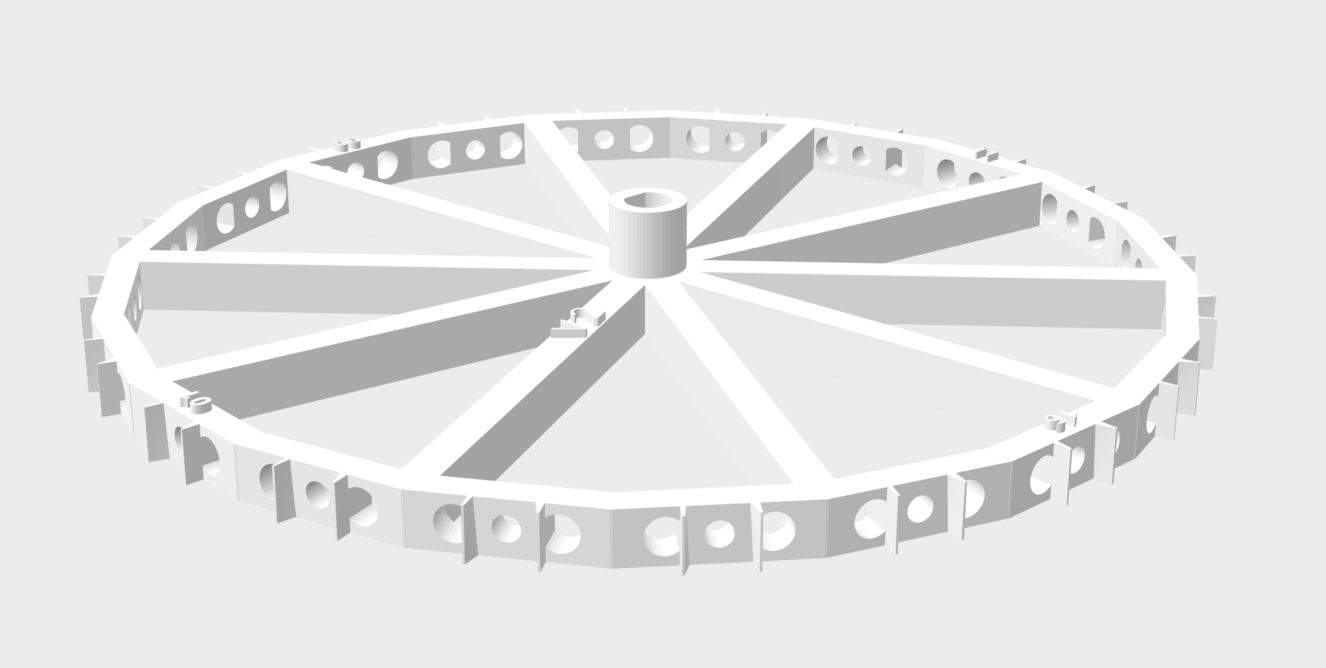
\includegraphics[width=5.208333in, keepaspectratio=true]{./fig/Camera_setup/Tool_Holder/Wheel_Holder/Second_Wheel_Holder/radhouder_v2.png}



In the wheel there are holes in which the clips fit. The center hole is as big as the hole in the inserts. This keeps the insert from moving round the hole.

The slads between the holes are made to fit the insert perfectly so this doesn't move or shift around. 



On the pictures the slads are visible which is not ideal so they will probably have to be adjusted in a future design.



The printing of these wheels was very difficult since it was with another material as we were used to and the print wouldn't stick to the print bed. This made a few bad runs and hours of wasted printing time. At the end 8 wheels of this are printed correctly and were used to create the Birthday dataset and the spaghetti dataset.



The clips looked like this:

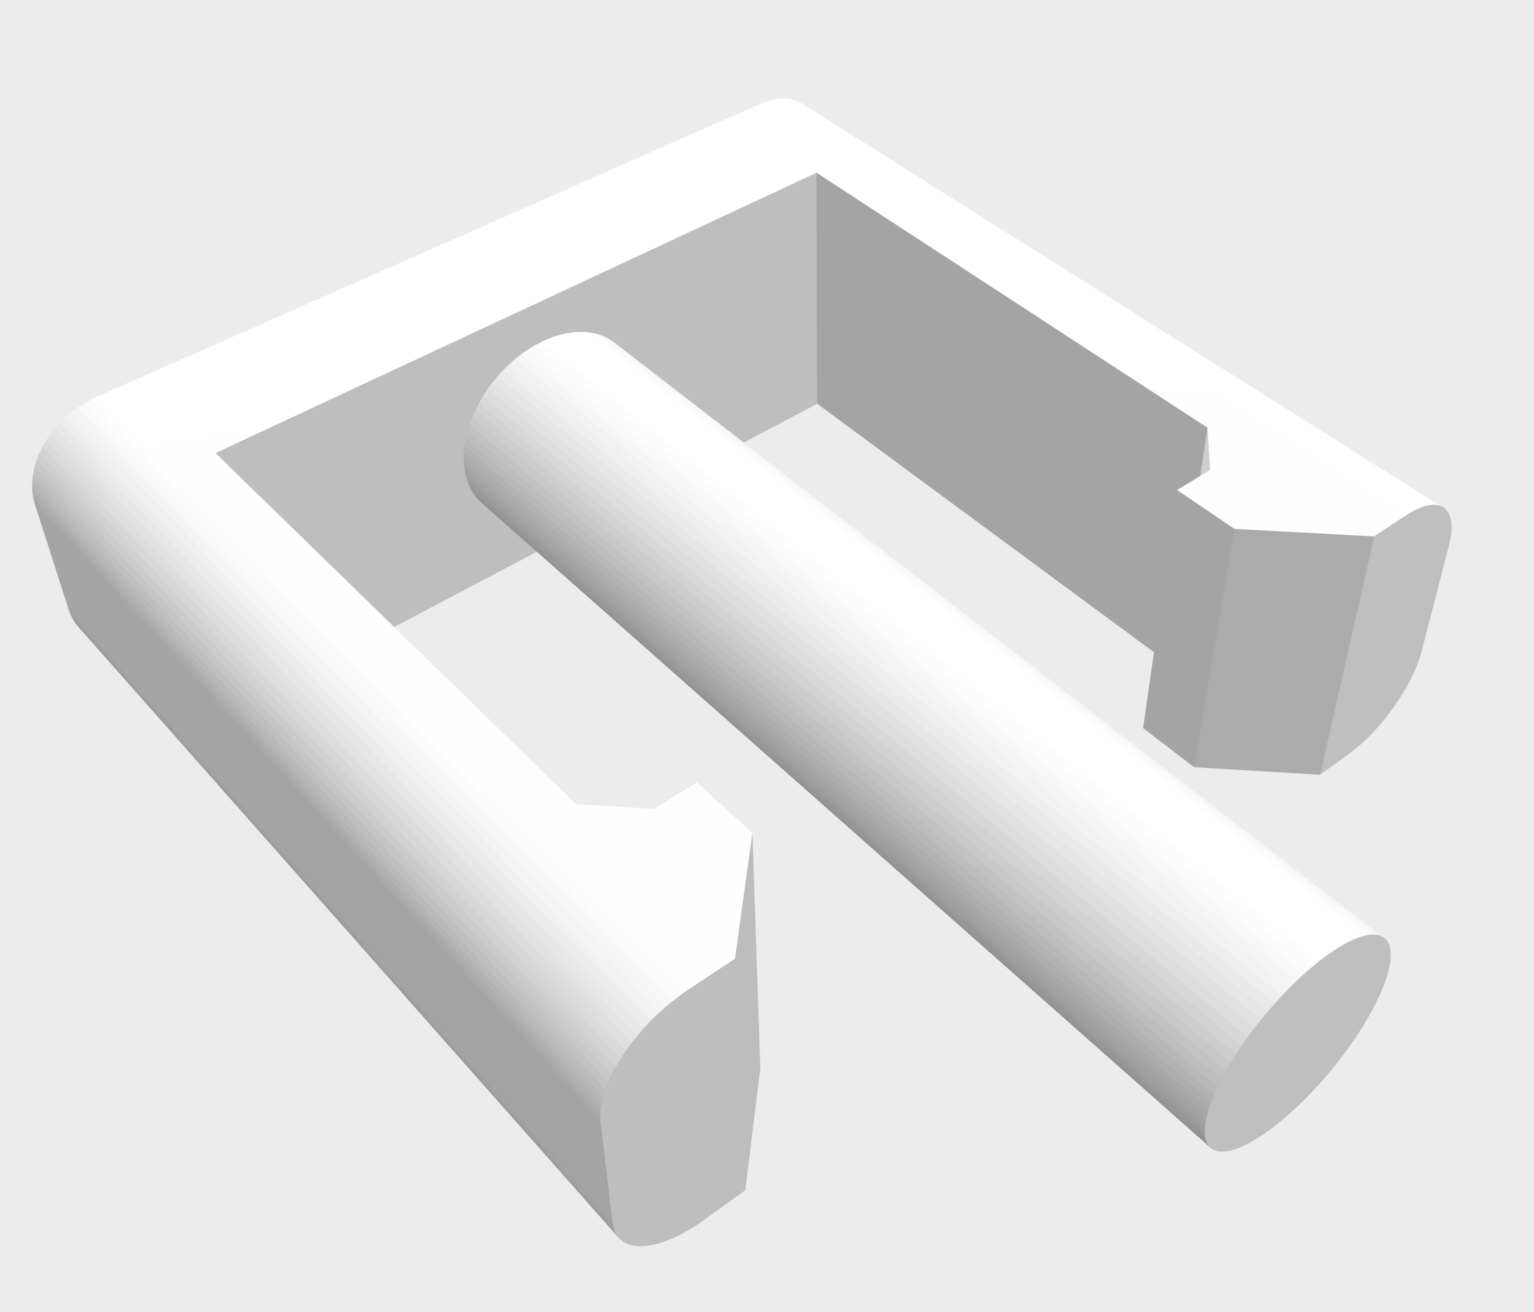
\includegraphics[width=3.125000in, keepaspectratio=true]{./fig/Camera_setup/Tool_Holder/Wheel_Holder/Second_Wheel_Holder/clip_9.png}
\subsection{Design different lighting solutions}

		\subsubsection{Light}

Created zaterdag 24 oktober 2020



Different light setups:

\begin{enumerate}
\item Desk Lamp
\item white led strips (long) 
\item  led strip (single led)
\item Color changeable led strip (multiple combined in a matrix)
\item top light (white or colored)
\end{enumerate}

\subsubsection{Adressable Color Changeable Led Strip}

Created Wednesday 28 October 2020



A third option of lighting is playing with the colors of the light. to archieve this a setup will be created with a single adressable light strip where the color and led can be freely chosen. 



To assign a color which works best; a study is made to find the wavelengths where the light reflects most on the used materials of the tool. This can be found in  Light Reflection


		\subsubsection{Desk Lamp Test}

Created Wednesday 28 October 2020



First test using following setup:



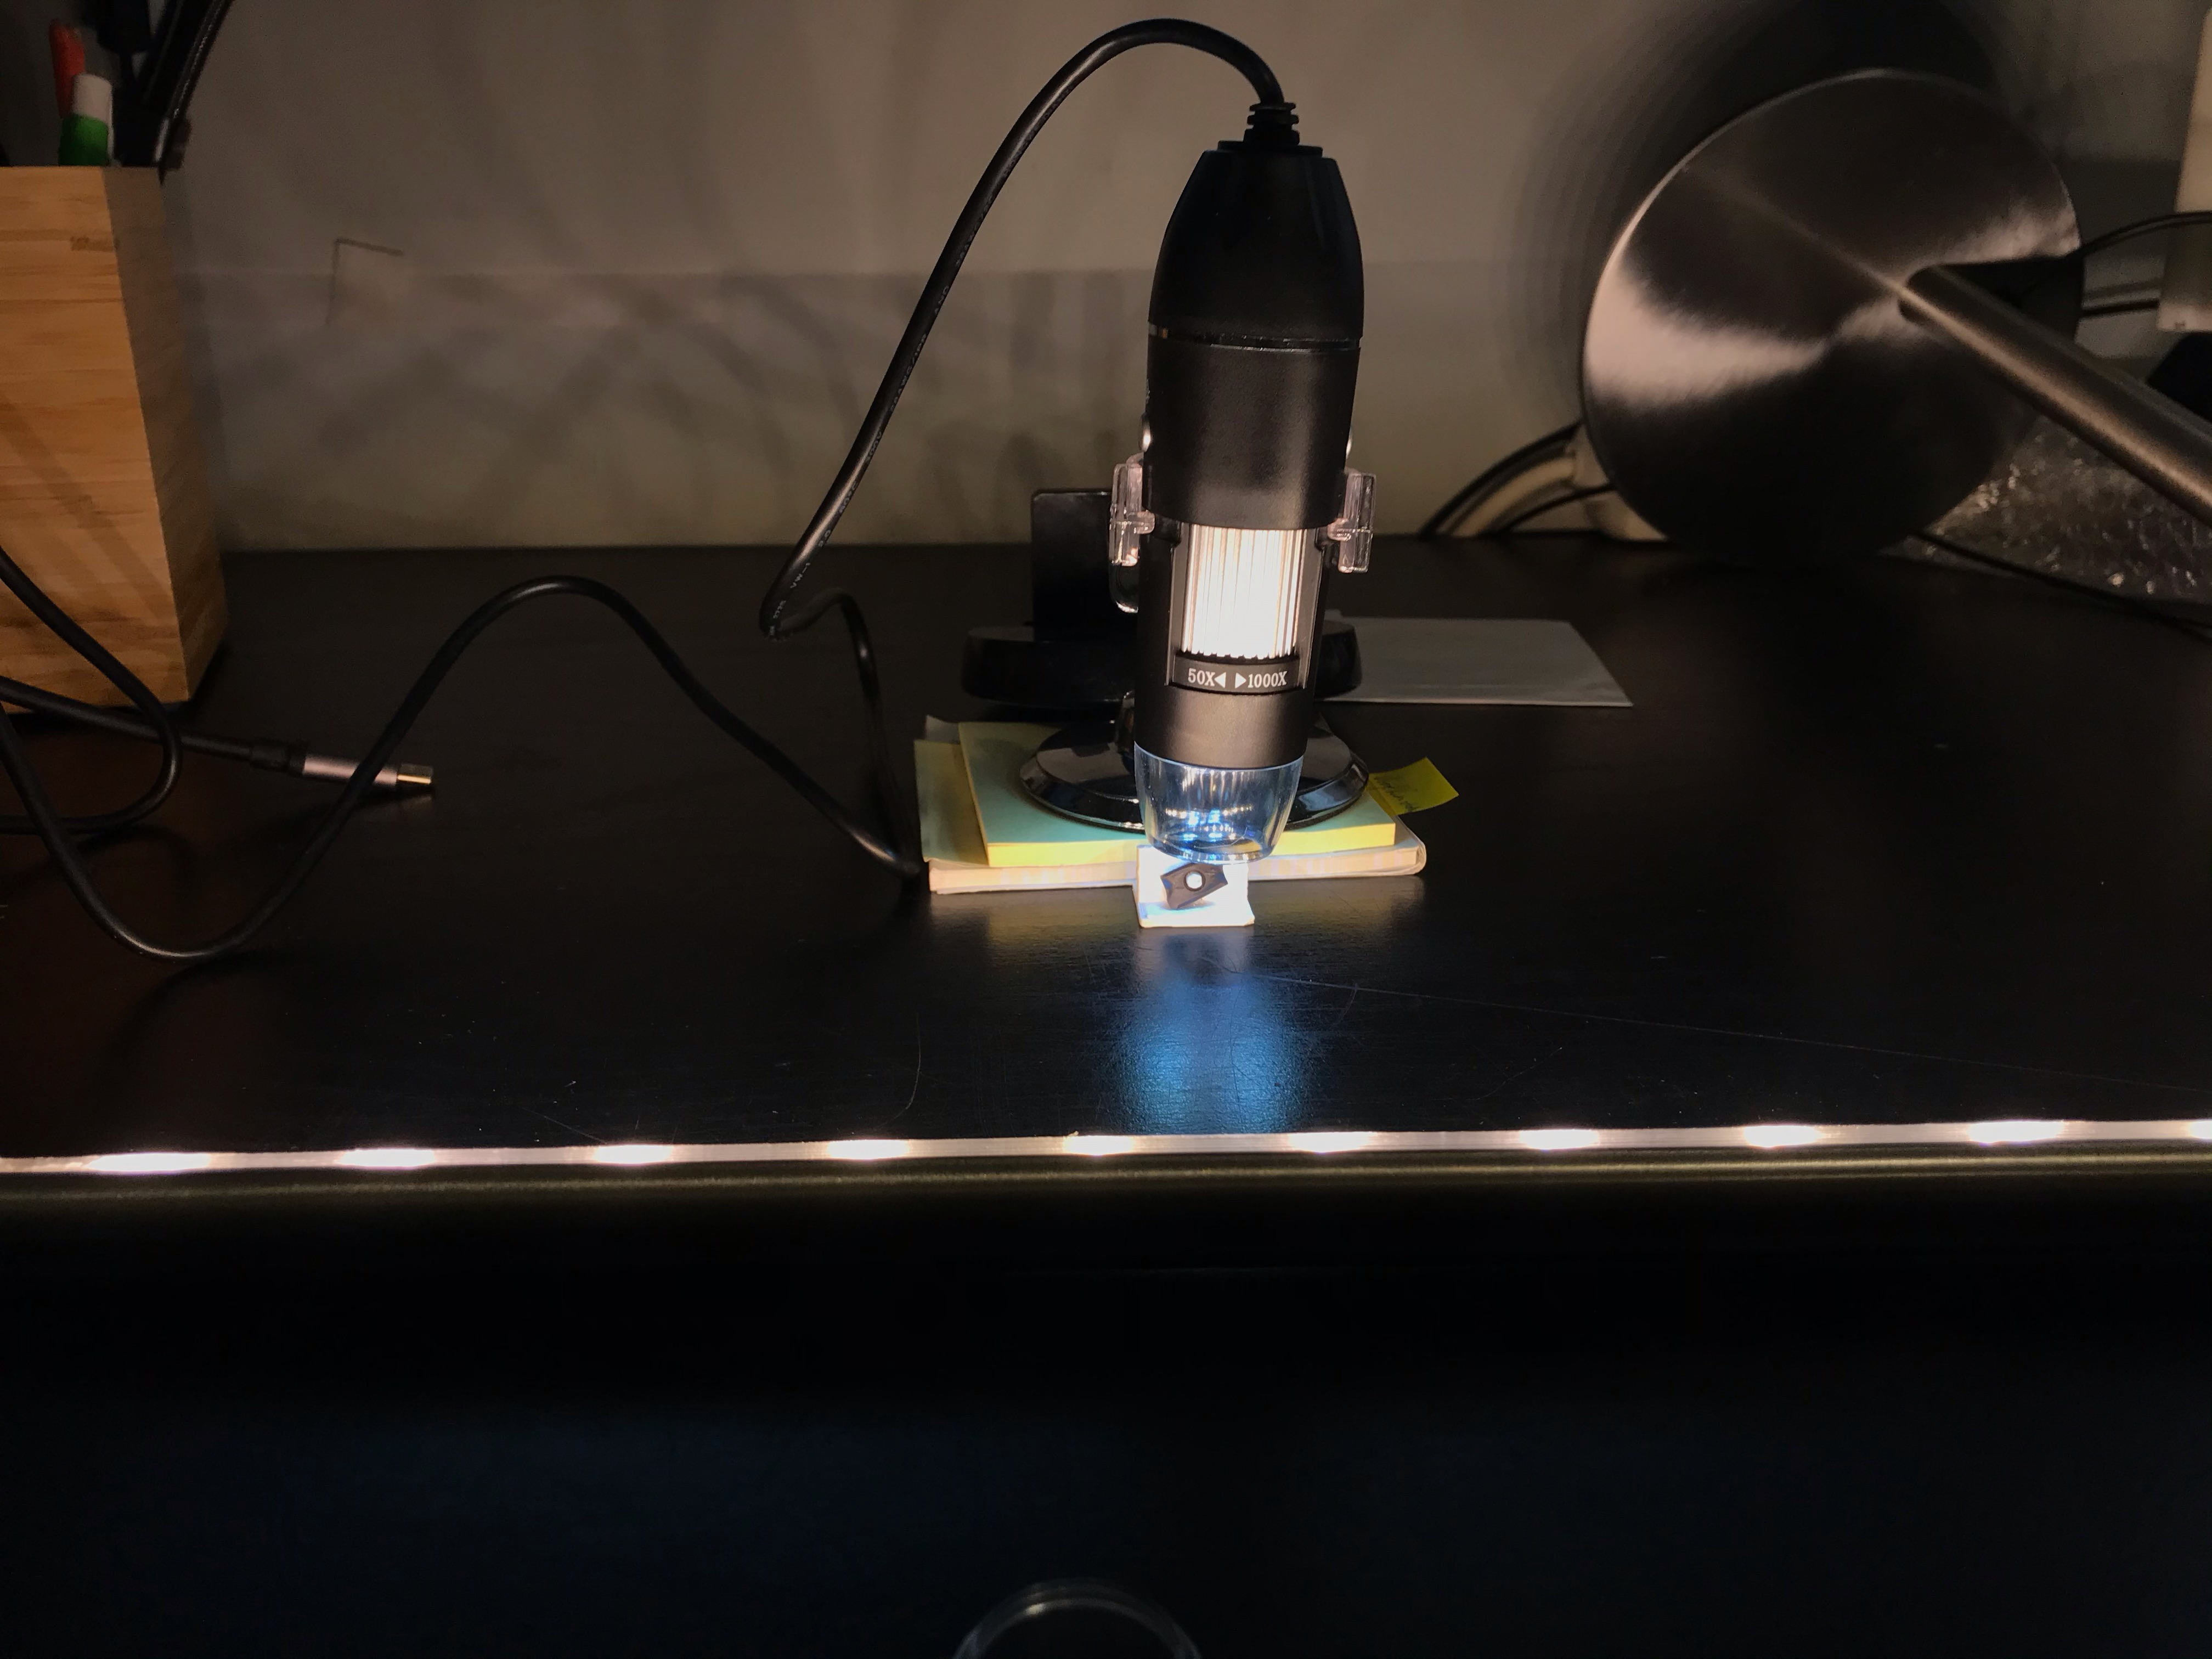
\includegraphics[width=4.166667in, keepaspectratio=true]{./fig/Camera_setup/Light/Desk_Lamp_Test/eerste_setup_andere_richting.jpeg}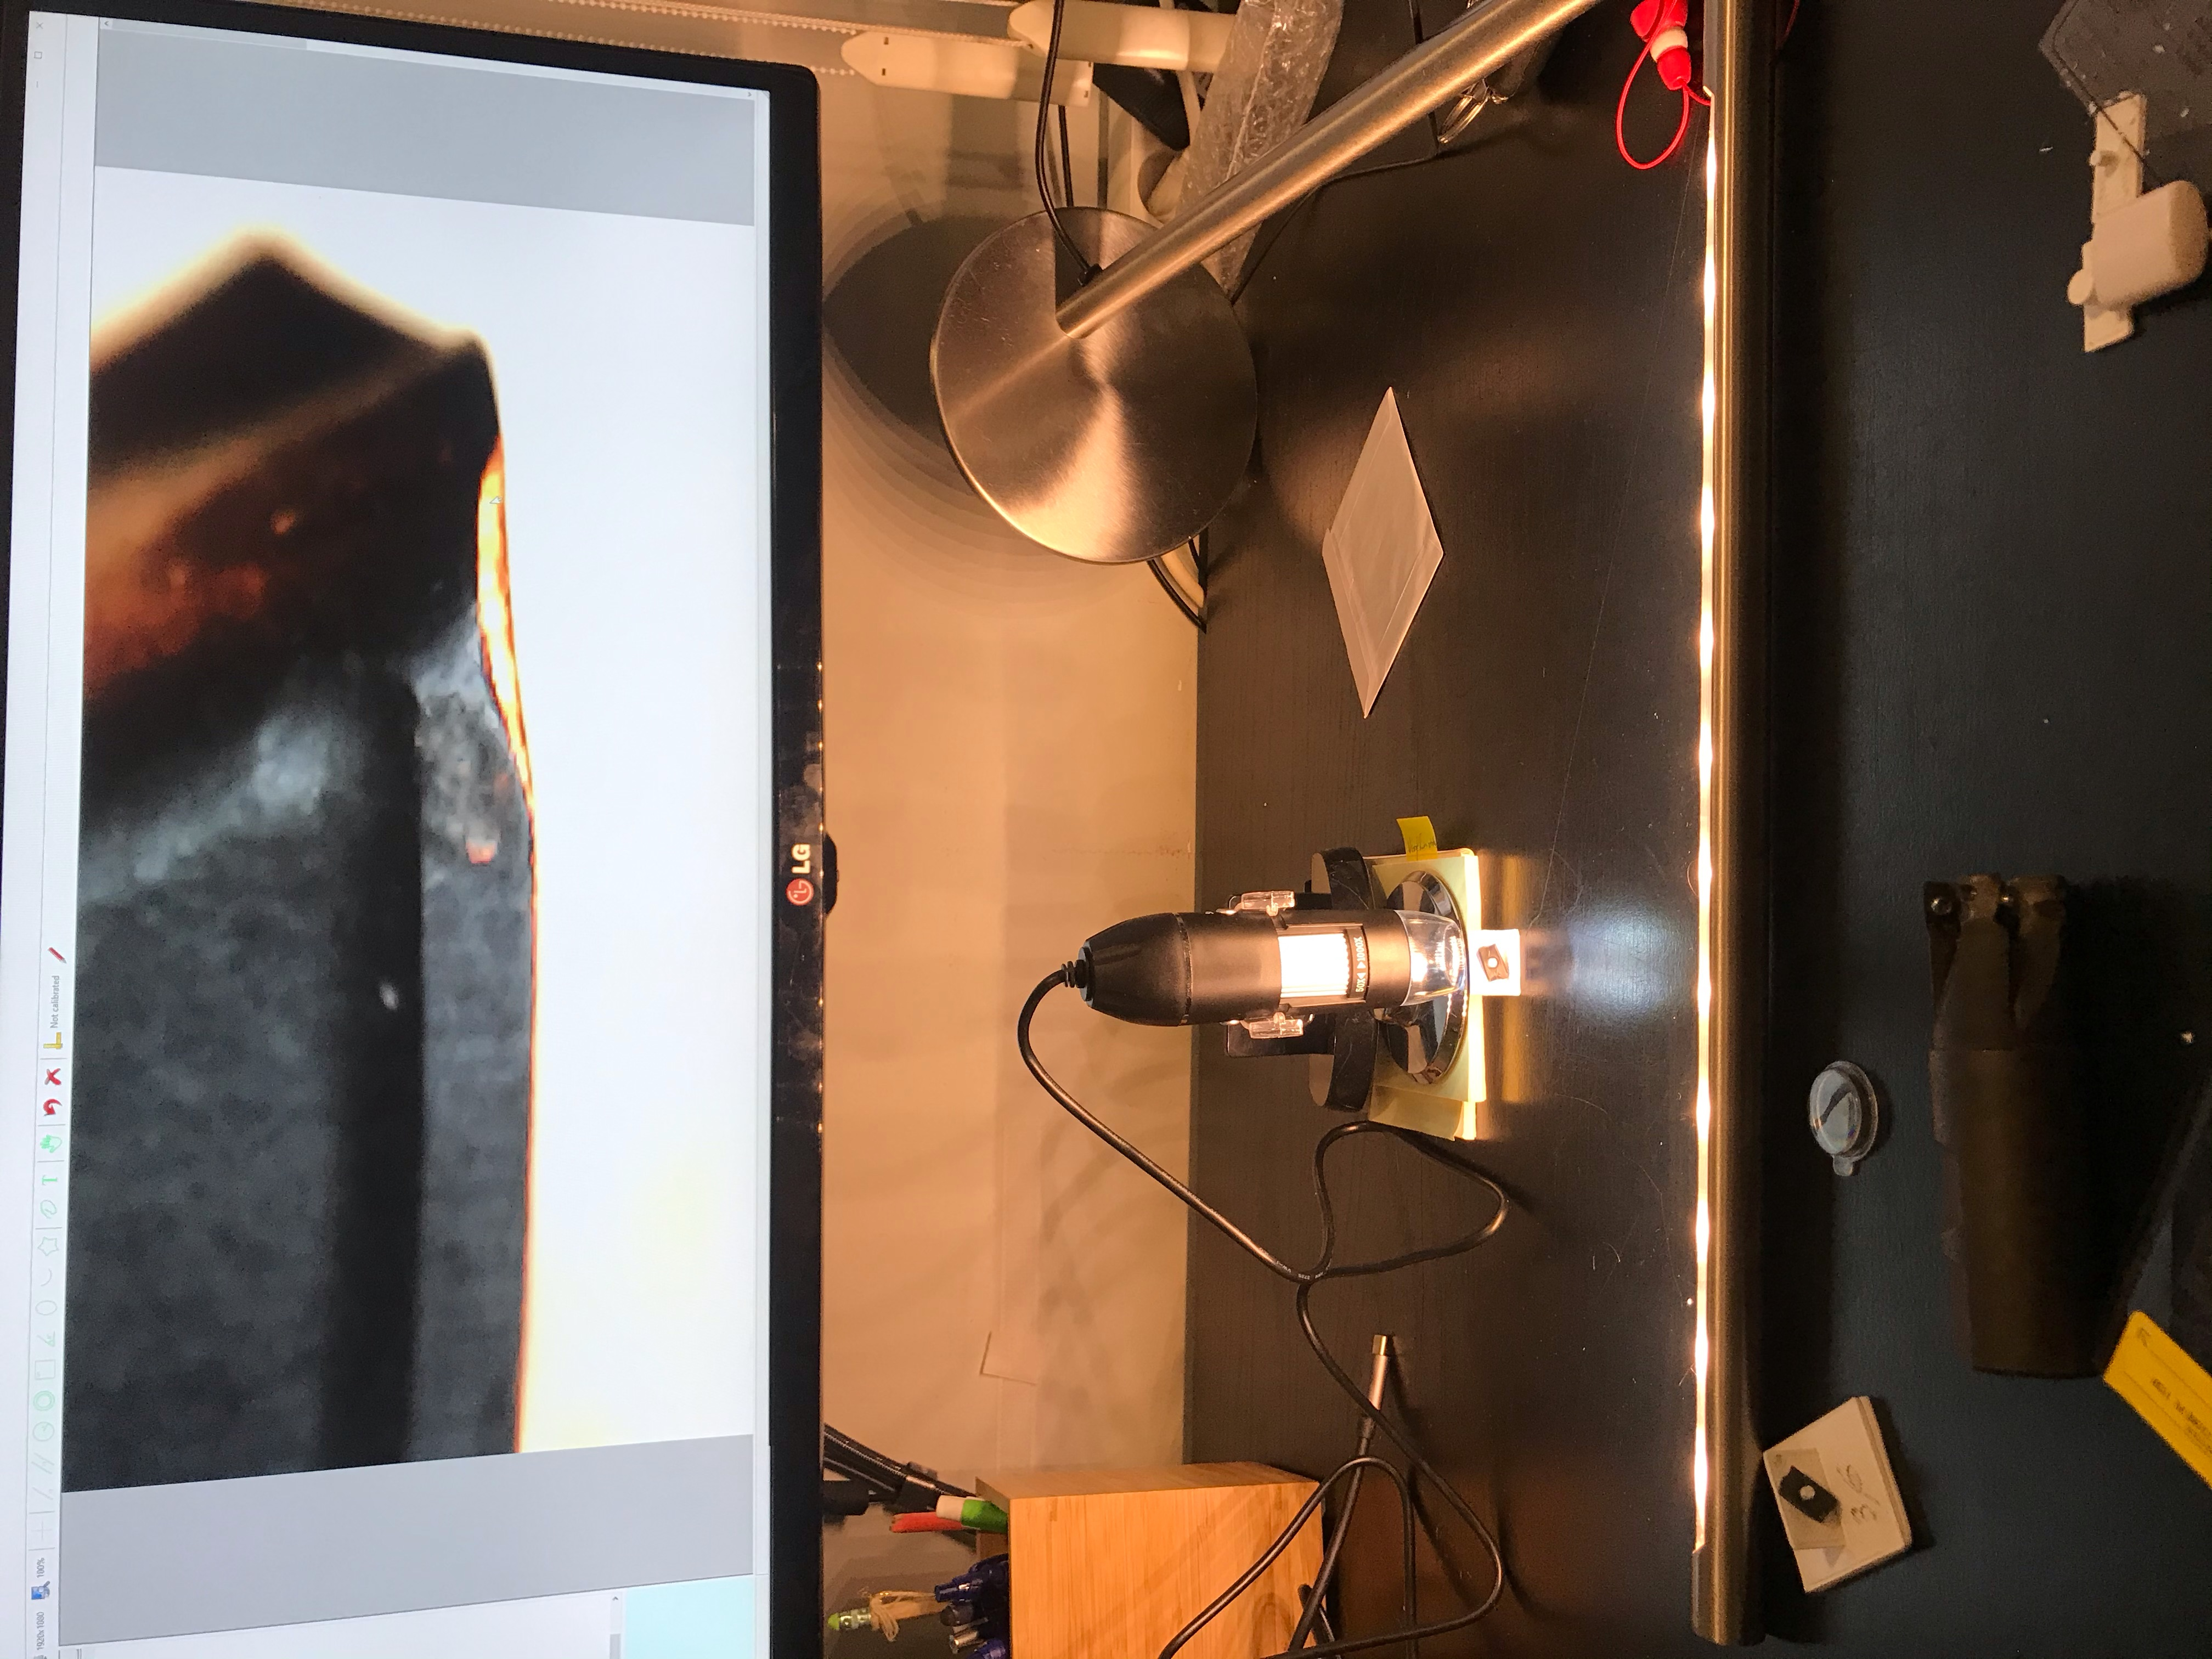
\includegraphics[width=4.166667in, keepaspectratio=true]{./fig/Camera_setup/Light/Desk_Lamp_Test/eerste_setup_andere_richting_beeld2.jpeg}



This setup was using the top light of the camera. This light was good to be able to adjust the camera. Without the light, the errornous places where more visible. But the desk lamp had to much brightness. Therefor and to test other lighting conditions a led strip will be used for further tests. 



The result with this setup can be seen in the above picture on the screen. here can be seen that there is a bright white background behind the tool. In a new setup there will be tried to make the background as dark as possible to make sure only the bad part of the tool is clearly lighted.



The result of this is shown in the following picture where the light is blocked off of the rest of the tool and only the errornous part is lightened. This would be a good start to start creating a dataset.



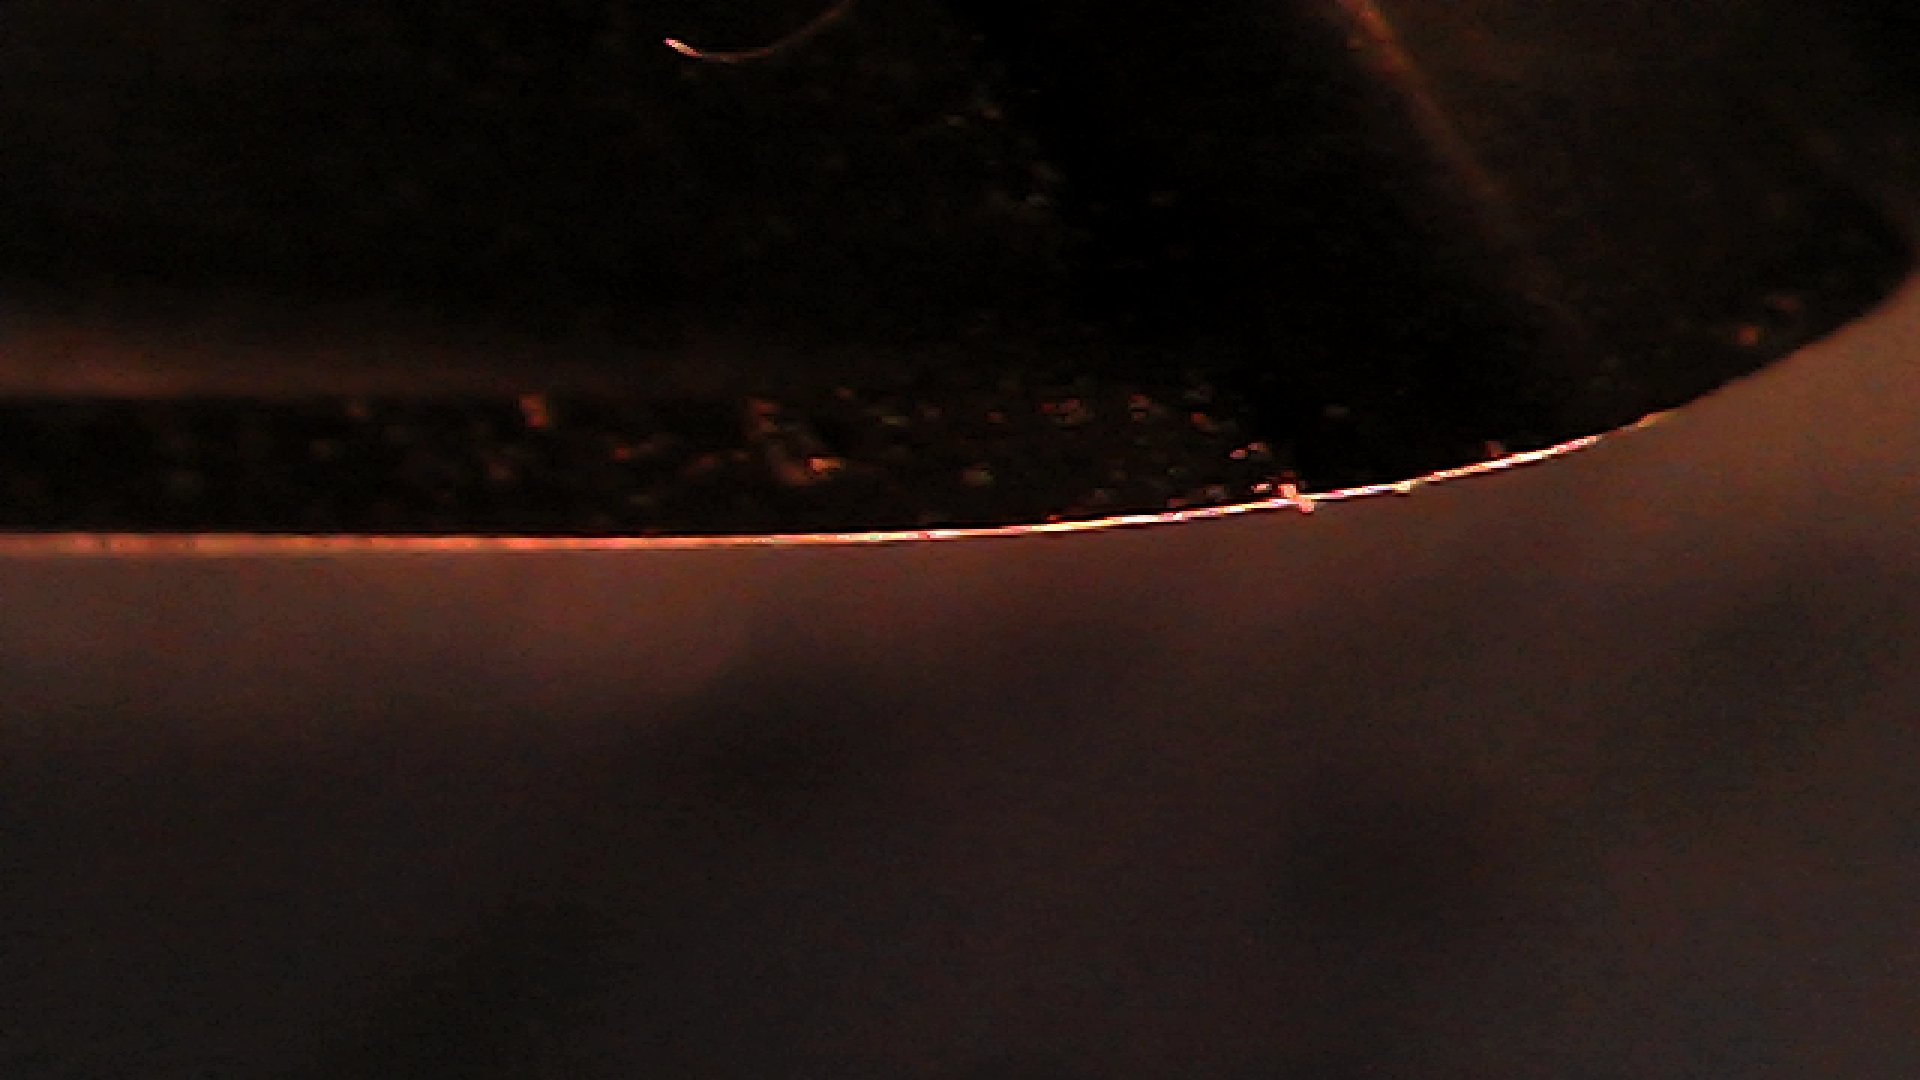
\includegraphics[width=4.166667in, keepaspectratio=true]{./fig/Camera_setup/Light/Desk_Lamp_Test/eerste-opstelling_donkere_achtergrond2.jpg}



The color of the desk light set a good gradient of bad vs good sets. White areas are worn very hard while orange is not worn that hard.



By tilting the lamp up and down in a horizontal way, all the areas where ligthtend. 



The setup used for this lighting scene is described 


		\subsubsection{White Led Strips}

Created Wednesday 28 October 2020



A second lighting contition created is the lighting with 3 the same led strips controllable with a raspberry pi. 

This was tested using some transistors to create a controllable switching circuit. This didn't work due to the wrong type of transistors. The second option is to control the led strips using proper relays. These will have to be bought separately so is must still be assessed if this is needed.



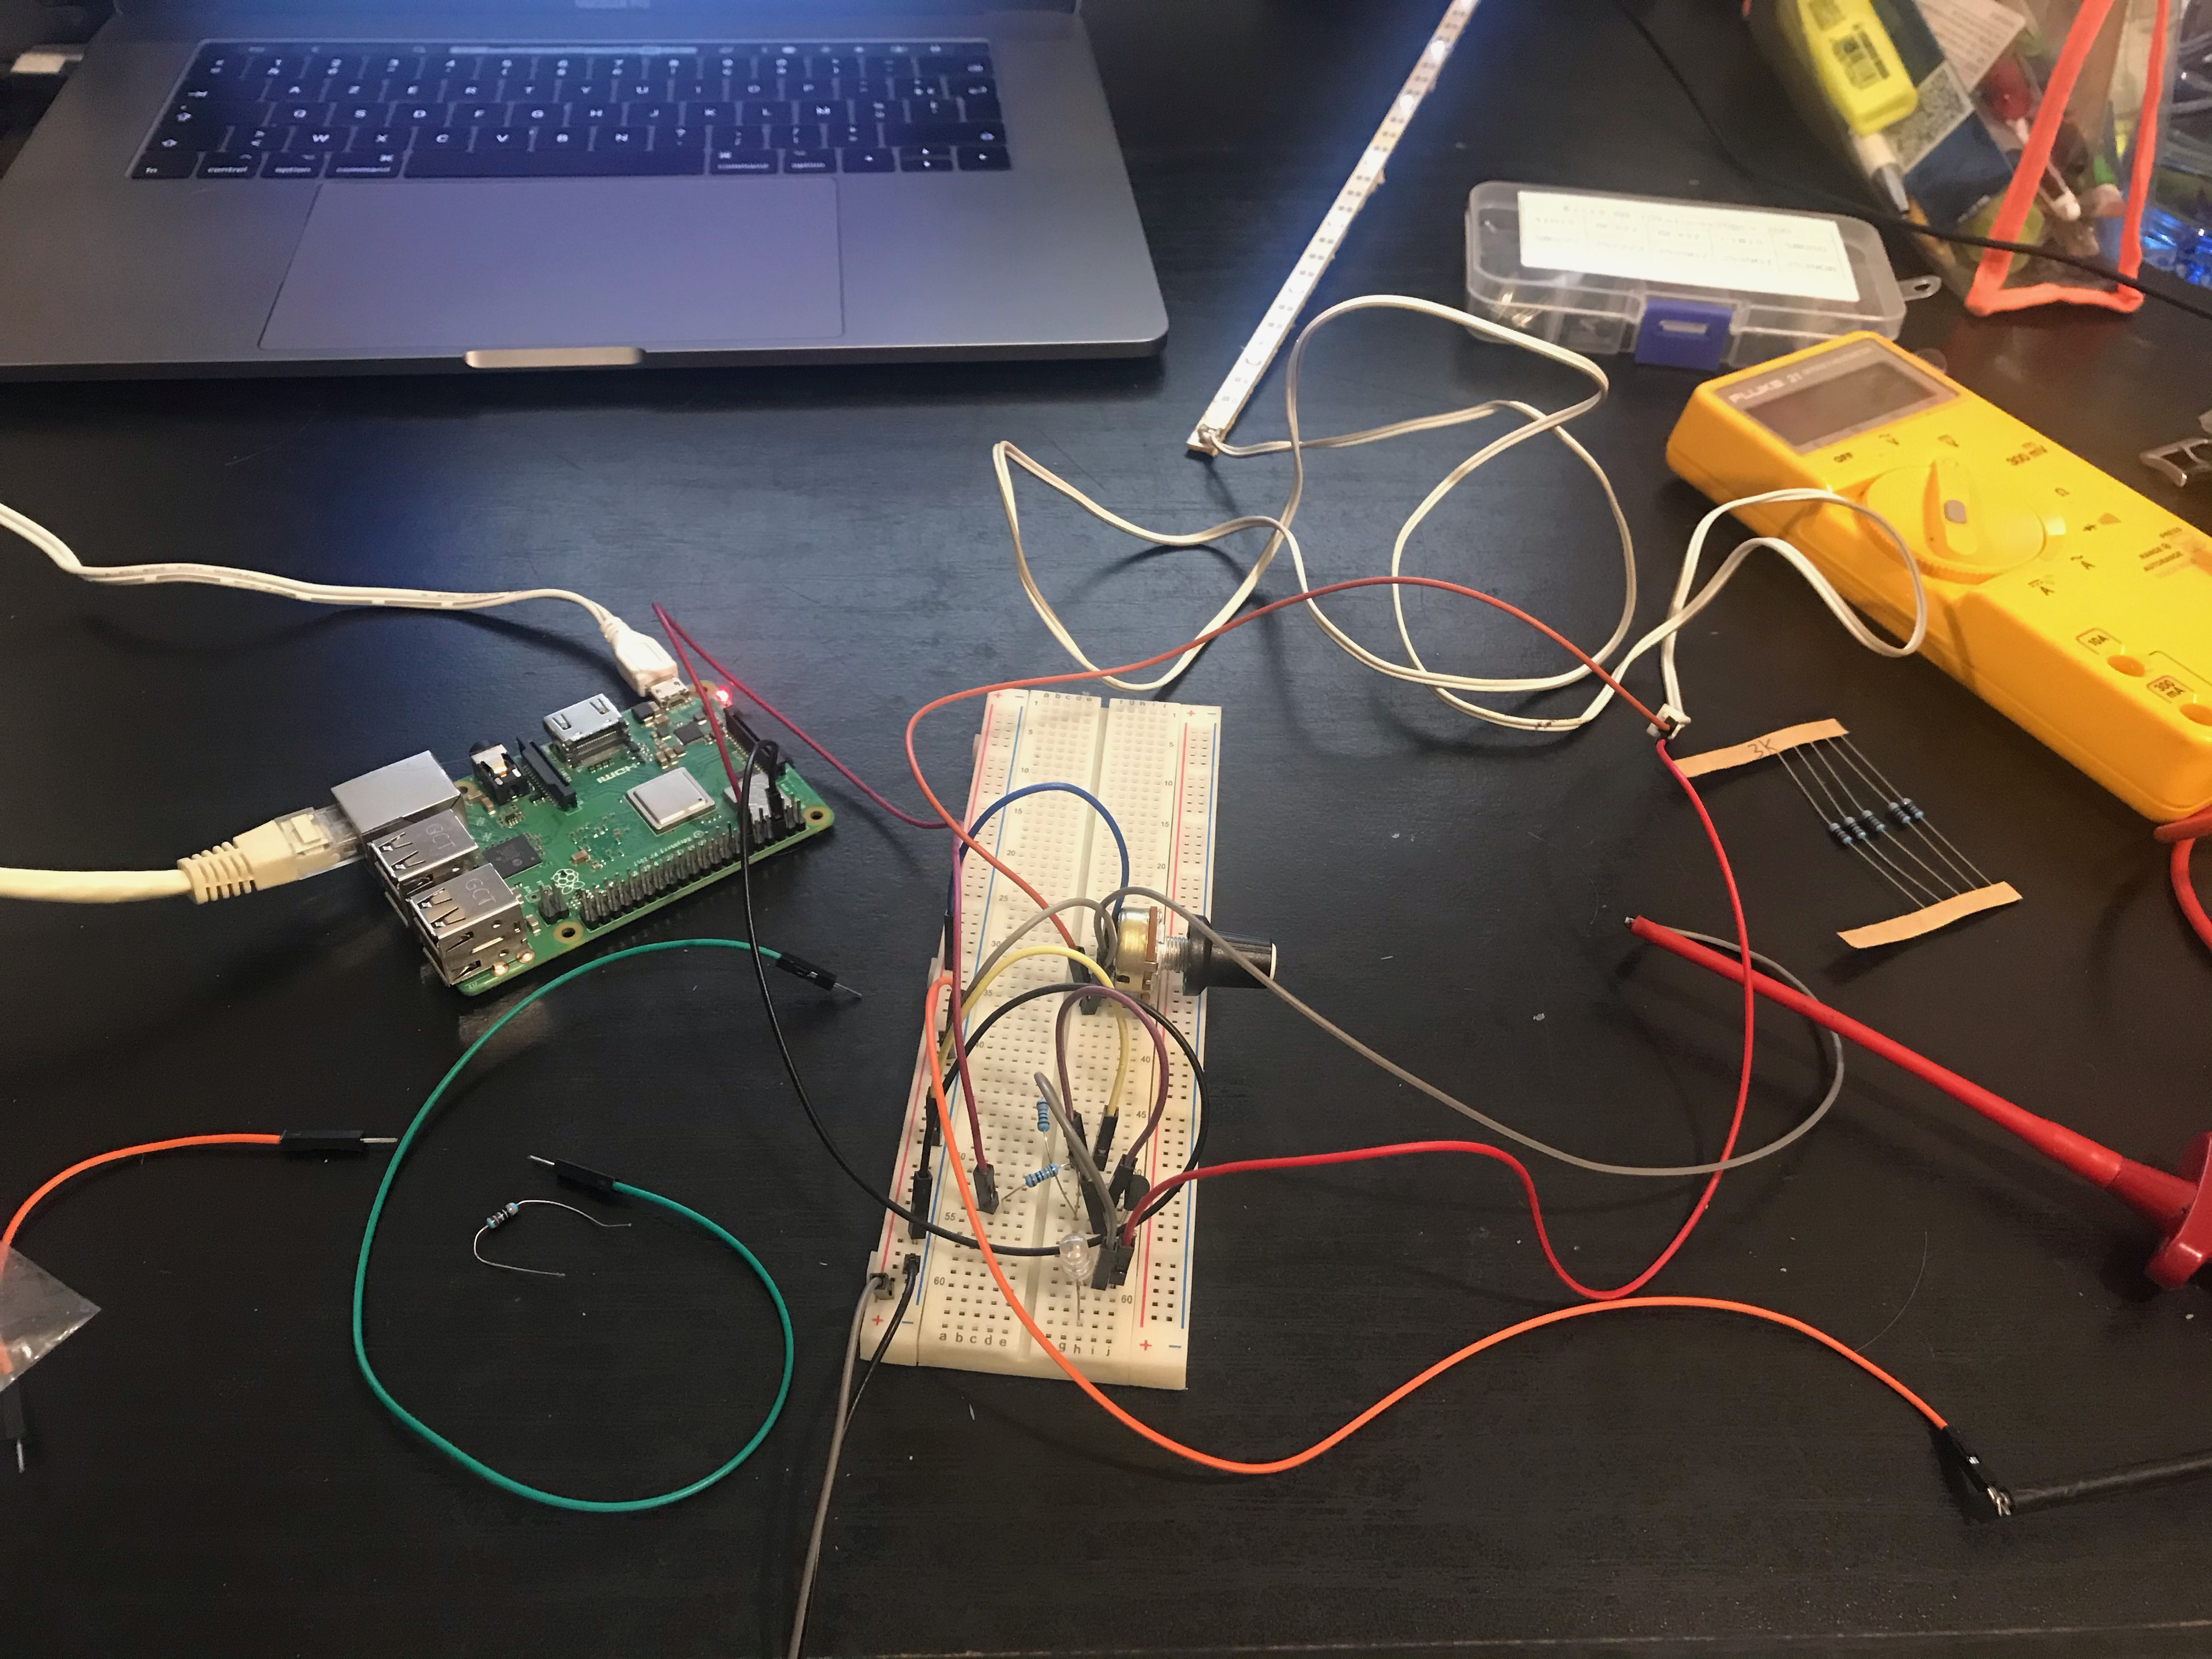
\includegraphics[height=3.125000in, keepaspectratio=true]{./fig/Camera_setup/Light/White_Led_Strips/Test_setup_ledstrip.jpeg}

The setup to test the control of a led strip using a NPN transistor as switch.

\subsection{Design a way to mount the camera in a desired spot}
		\subsubsection{Camera mount}

Created Wednesday 28 October 2020



In this page the camera mount will be discussed along the design process of the setup



\begin{enumerate}
\item Holder 
\item Wheel holder
\end{enumerate}

\section{Vision Algorithm}

\subsection{Finding an algorithm to test the camera position setup}

First there must be found an algorithm that can quickly confirm wether a setup is good or not. This will be done by taking pictures different camera positions with the same lichting. After this the images go trough a simple model and the output is verified with a test set. 

This algorithm must be as small as possible to not have to take a lot of pictures to determine wether an algorithm is good or not. 

\section{camera position validation}

Created woensdag 18 november 2020



\subsection{Information}

The next data input structure is made:

	\begin{itemize}
	\item 20 train images
	\item 10 validation images
	\item 10 test images
	\end{itemize}


These images will go through different algorithms multiple times and the outputs are verified for every different algorithm.



\subsection{papers}



\begin{enumerate}[1]
\item A Comprehensive Study on Deep Image Classification with Small Datasets
	\begin{enumerate}[a]
	\item short comparison of the amount of convolutional layers to be used in the network (5 is optimal)
	\item comparison on datasets: Caltech101, CIFAR10
	\item also transfer learning also around 5 convolutional layers is the optimum
	\item network architecture
		\begin{enumerate}[1]
		\item from scratch:
		\end{enumerate}
	\end{enumerate}
\end{enumerate}
			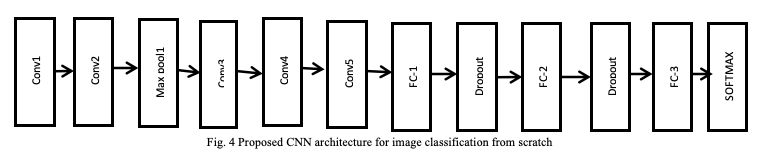
\includegraphics[]{./fig/Research/Vision_Algorithm/camera_position_validation/paper1_arch_fromscratch.png}
			
		\begin{enumerate}[1]
		\setcounter{enumi}{1}
		\item transfer learning pretrained on VGG16 with imagenet dataset
		\end{enumerate}
			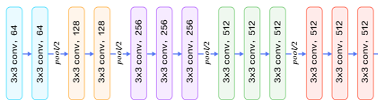
\includegraphics[]{./fig/Research/Vision_Algorithm/camera_position_validation/paper1_arch_transferlearning.png}
			
\begin{enumerate}[1]
\setcounter{enumi}{1}
\item Deep learning for image classifification on very small datasets using transfer learning
	\begin{enumerate}[a]
	\item creation of an image classification network with context of where it comes from
		\begin{enumerate}[1]
		\item alexnet vs googlenet vs vgg and the history
		\item displays keras code to create the same models
		\item architecture for models is shown
		\item niet super interessant gezien hier nog steeds wordt gewerkt op 6000 fotos van katten en honden, wel een indicatie dat deep learning gaat met weinig data
		\end{enumerate}
	\end{enumerate}
\end{enumerate}




\begin{enumerate}[1]
\setcounter{enumi}{2}
\item \href{https://paperswithcode.com/task/small-data}{https://paperswithcode.com/task/small-data}
	\begin{enumerate}[a]
	\item interesting papers with small datasets
	\end{enumerate}
\end{enumerate}


\begin{enumerate}[1]
\setcounter{enumi}{3}
\item A survey of the recent architectures of deep convolutional neural networks
	\begin{enumerate}[a]
	\item overview of almost all neural networks with their strengths and weaknesses
	\end{enumerate}
\end{enumerate}


\begin{enumerate}[1]
\setcounter{enumi}{4}
\item SDD-CNN: Small data-driven convolution neural networks for subtle roller defect inspection
	\begin{enumerate}[a]
	\item very interesting paper detects faults in bearing rollers. 
	\item Using very little data
	\item results with from scratch training best with SDD-inception v3 and SDD-resnet18
	\item SDD-VGG16 gets good results, but with long trainin time
	\end{enumerate}
\end{enumerate}


In most seen papers a very low learning rate 

0.0005 

\section{Datasets}

Created vrijdag 13 november 2020



A separation is made between hand made datasets and automated datasets because they take a very different approach and produce very differing pictures.



\subsection{Handmade datasets}

The following datasets where produced using a microscopic camera to take pictures of single inserts all placed under the camera by hand.



\subsubsection{initial dataset}

	The initial dataset where the images made by a microscopic camera at Sirris. These pictures were taken for the measurement of the toolwear. This dataset provided the labels for the first 5 batches labeled with 00x.
	


\subsubsection{Second handmade dataset}

	A second dataset was made to compare the pictures with the previous dataset. This is done to verify the images and the results and to determine 	what the marker meant. This dataset also handles the first 5 batches labeled with 00x
	


\subsubsection{second initial dataset}

	The second initial dataset was made with the inserts from batches 11 to 19 labeled with 01x. Here the images where taken with the same microscope as the first initial dataset but instead of phtotographing only the one insert at a time; two inserts are photographed per shot.
	


\subsection{Automated datasets}

First the camera position is discussed and than the datasets are all listed.



\subsubsection{Camera position}

	This discussed two setups where on the one the camerea is more pointed to the side of the insert and the other one is pointed more to the top of the insert.
	
	\begin{enumerate}[1]
	\item 1 camera position side dataset
	\item 2 camera position top dataset
	\end{enumerate}


\subsubsection{created datasets}

	All created datasets which conduct a few images that are worth processing are discussed here. 
	


	\begin{enumerate}[1]
	\item birthday dataset
		\begin{enumerate}[a]
		\item conducted tests
		\end{enumerate}
	\item Spaghetti dataset
		\begin{enumerate}[a]
		\item conducted tests
		\end{enumerate}
	\end{enumerate}

		\section{automated datasets}

Created vrijdag 04 december 2020



Divided in a few topics:



\begin{itemize}
\item check camera position which will discuss different camera position angles
\item created datasets where all fully created datasets will be discussed
\end{itemize}

		\section{1 check camera position}

Created vrijdag 04 december 2020



\subsection{1 \$ 2}

In this set there will be defined what the best camera position is for the creation of the dataset. Top view as well as side view will be checked.


		\section{1 camera position side}

Created woensdag 11 november 2020



\subsection{Camera position on the side}

Taken on the first 4 plates of batch 04 with red lighting only from the adressable led strips. 



1st light position is made with a setup with two led strips where one image is taken for every set of two led lights. 

output is bad. Reflection angle wasn't good. 

Results saved in next directory

/Users/larsdepauw/Documents/Lars.nosync/Documents/School/1Ma ing/Masterproef/Images/dataset/First\_automated/camera\_zijkant\_dual\_ledstrip



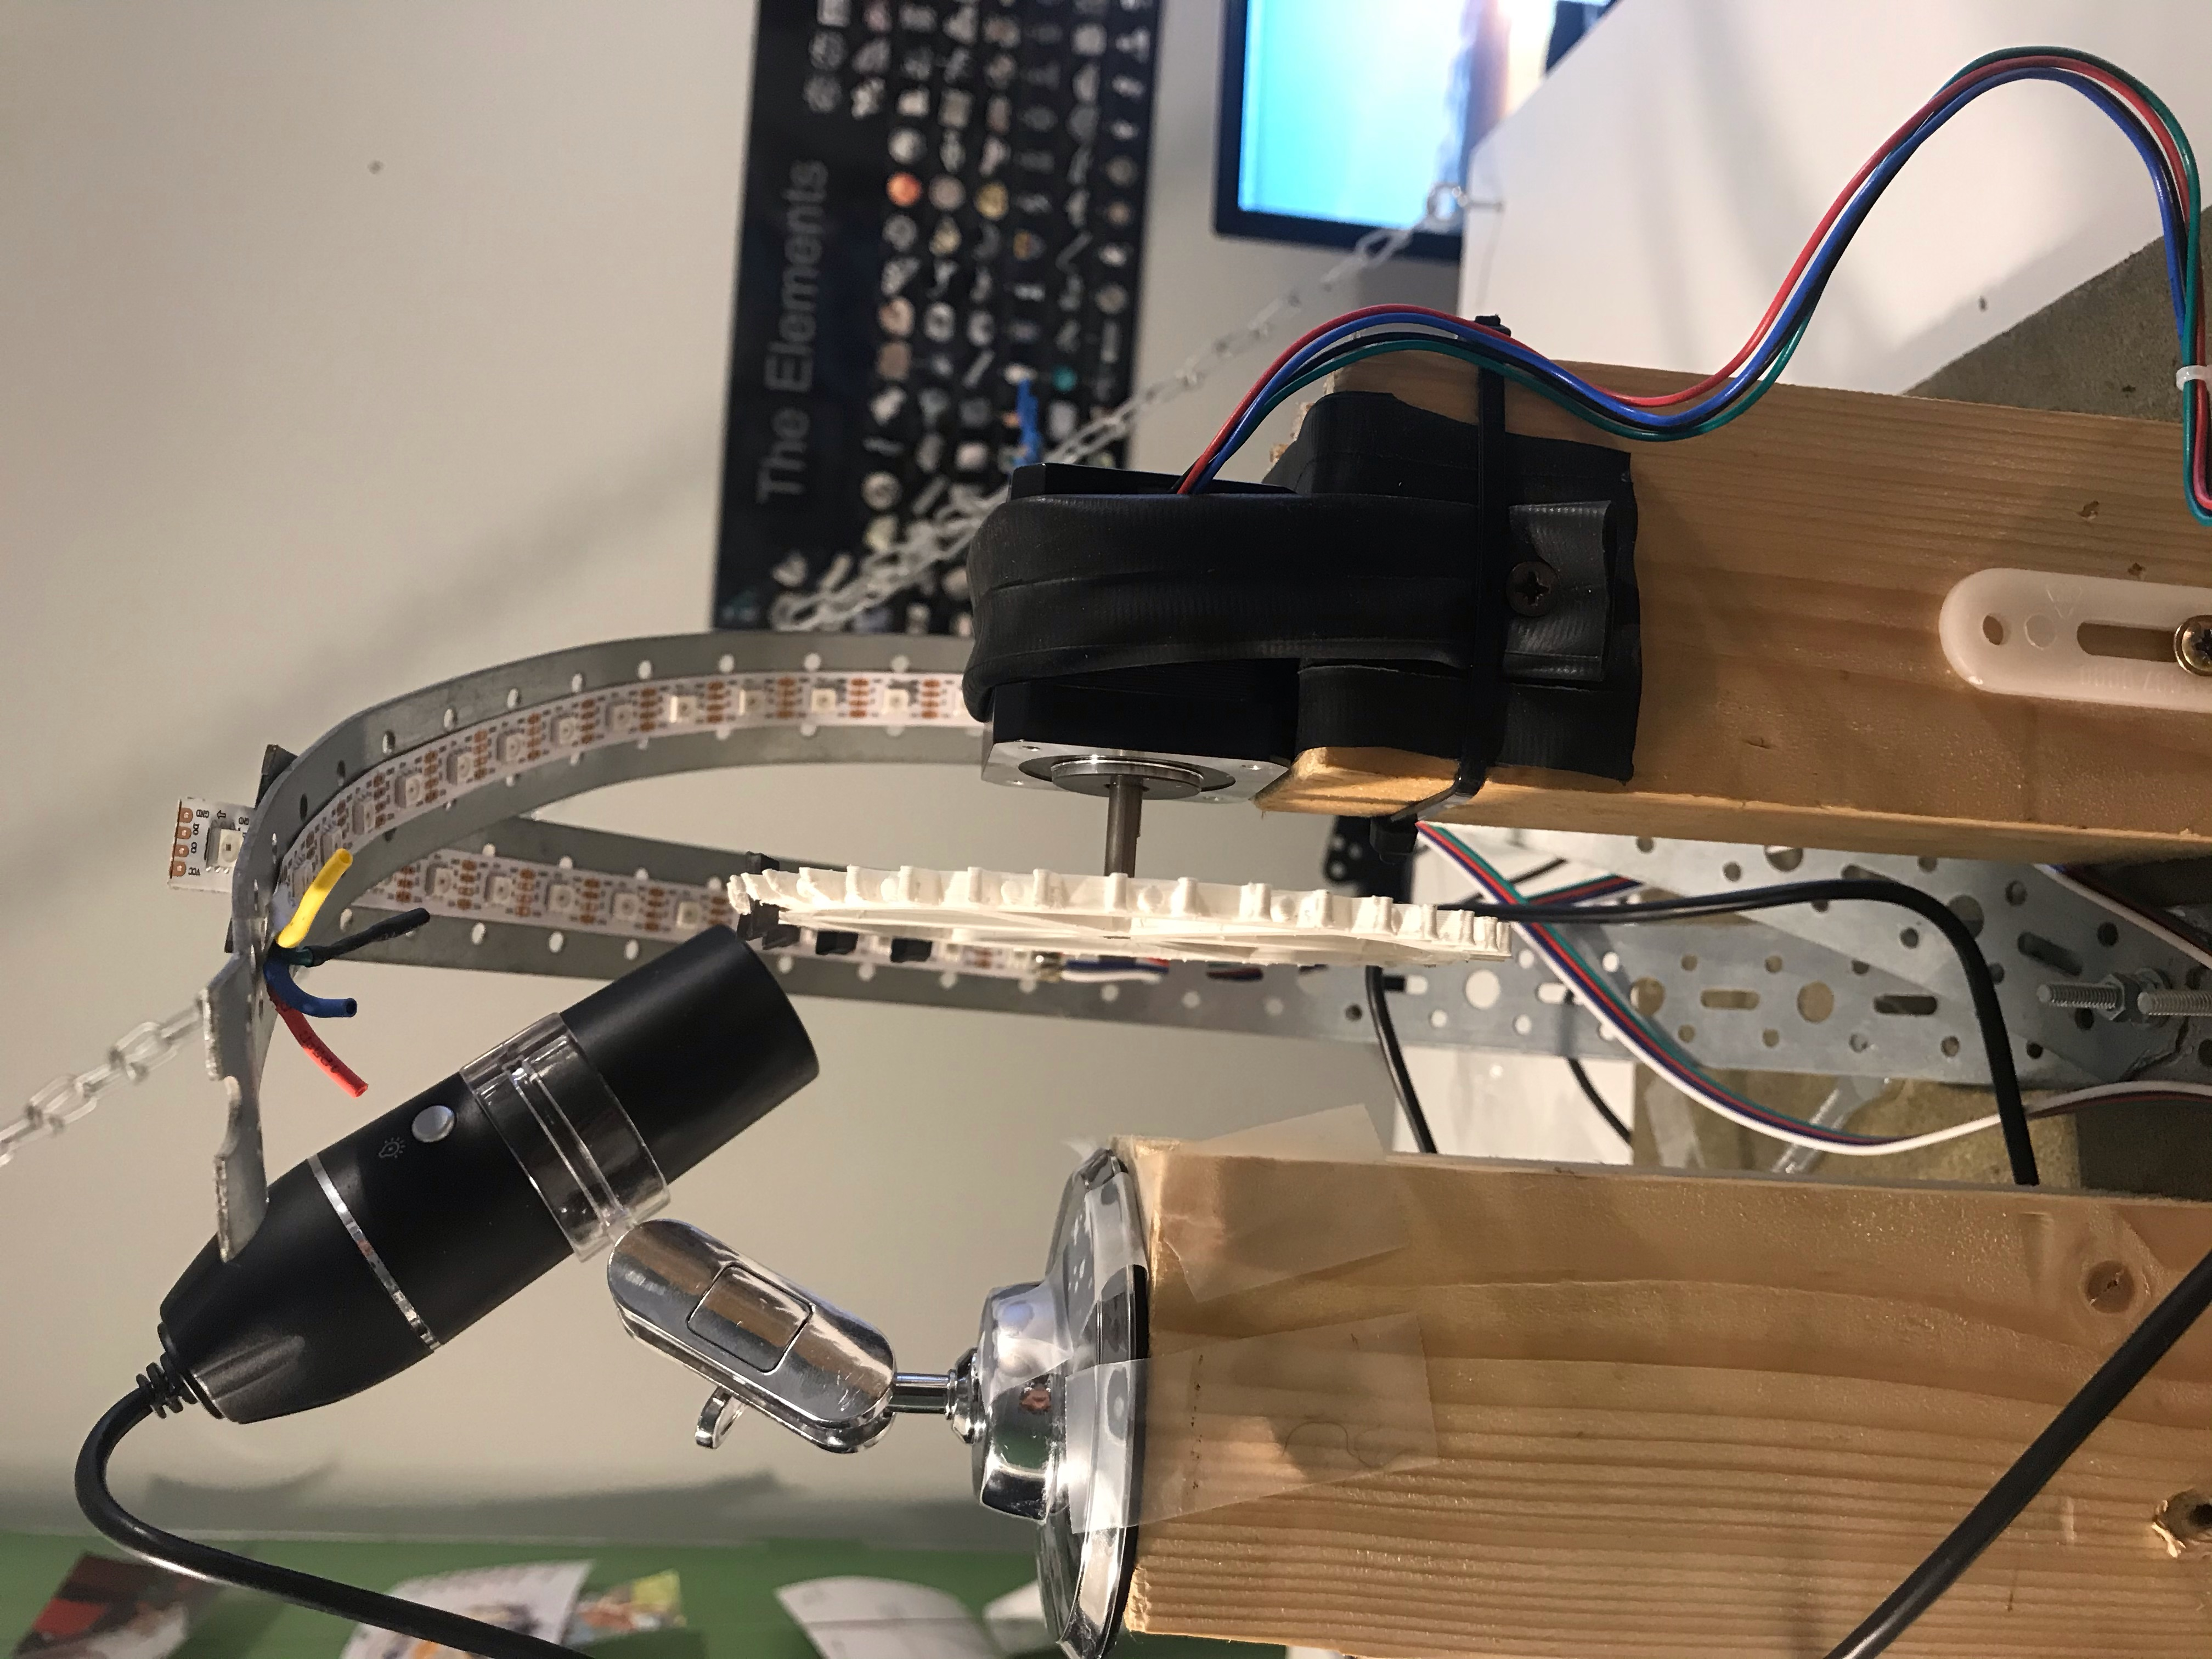
\includegraphics[width=4.166667in, keepaspectratio=true]{./fig/Vision/Dataset/automated_datasets/1_check_camera_position/1_camera_position_side/achter2.jpeg}



The images that where taken with this setup are found here:

Due to the problems with the arduino communications described here the first dataset wasn't successfull because the leds didn't turn on when the photo's where taken. So the results are all black pictures with al little shadow of the insert caused by the polluting light. 




\includegraphics[width=4.166667in, keepaspectratio=true]{./fig/Vision/Dataset/automated_datasets/1_check_camera_position/1_camera_position_side/p3_l6_black.png}



\subsection{Camera position on the side take two}



A delay was entered before sending a command to the arduino to provide the wanted lighting conditions. Although this was a very long process the results are way better than the ones from the first take on this camera setup. 



The same setup was used with the camera in the same position. For red led only the following image is the result.



The leds shown here leds 8 through 10. There is a nice lighting of every part of the wear

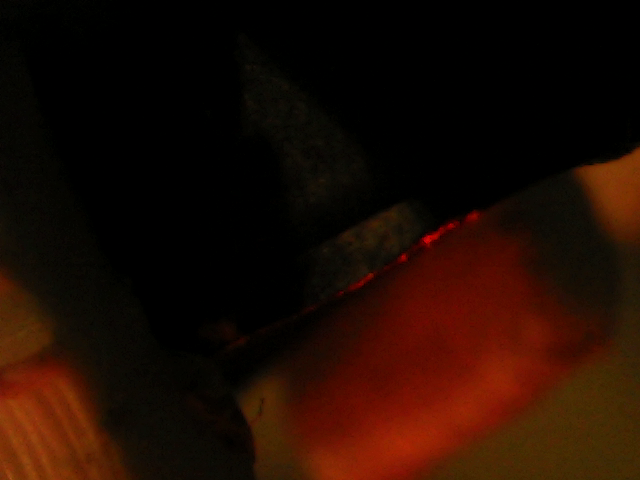
\includegraphics[width=3.125000in, keepaspectratio=true]{./fig/Vision/Dataset/automated_datasets/1_check_camera_position/1_camera_position_side/p3_l8.png}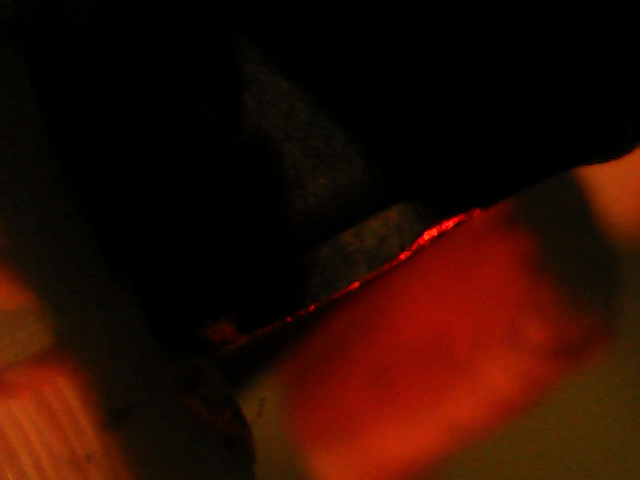
\includegraphics[width=3.125000in, keepaspectratio=true]{./fig/Vision/Dataset/automated_datasets/1_check_camera_position/1_camera_position_side/p3_l9.png}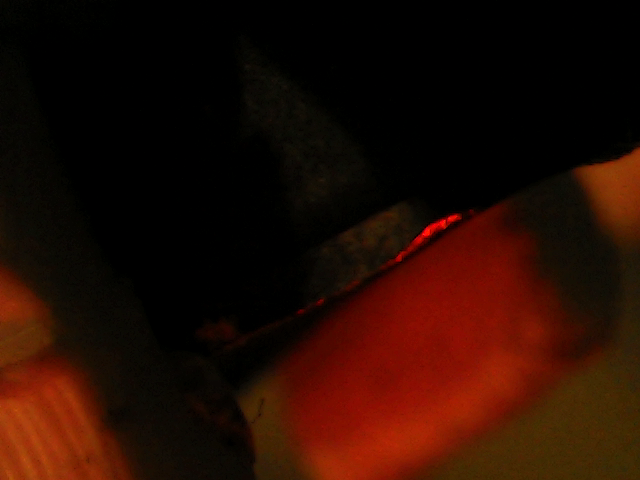
\includegraphics[width=3.125000in, keepaspectratio=true]{./fig/Vision/Dataset/automated_datasets/1_check_camera_position/1_camera_position_side/p3_l10.png}



This lightens the worn area very good. Although th ebackground is lighted as well and makes it harder to only see the worn area. On this we can build the first dataset. 

Next the top view was tested 


		\section{2 camera position top}

Created woensdag 11 november 2020



The same plates where used 04 -\textgreater{} 1until 5. 

Every pair of led is lighted separately to generate the photo's 



extra documents of the results in the folders images/dataset/.....



\subsection{Camera position to top}

The second test was conducted with the camera mounted a little more to the top of the inserts. This made the reflection from the worn area to the camera better. 

The first test results where also all black pictures caused by the same problem as on the first test of camera position side. On a second test this issue was resolved and the following pictures where the result. The issue was resolved by adding enormous amounts of delay for each command sent to the arduino. This made the process take very long (about 1 second per photo).



One picture was taken for every two leds of the strip with red light. for batch number 4 insert 3 with leds 5,6 and 7 turned on.



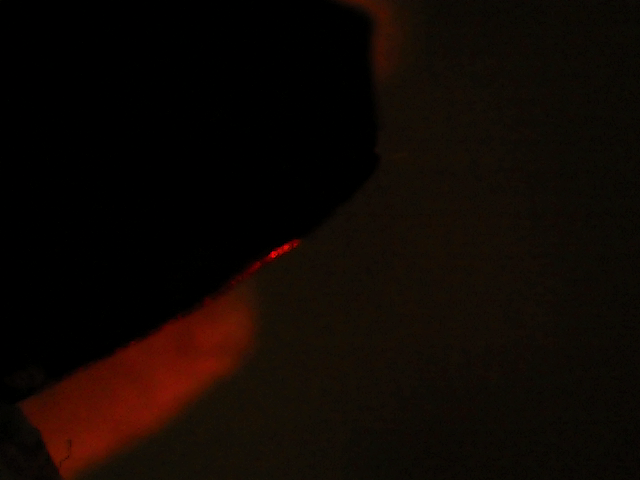
\includegraphics[width=3.125000in, keepaspectratio=true]{./fig/Vision/Dataset/automated_datasets/1_check_camera_position/2_camera_position_top/p3_l5.png}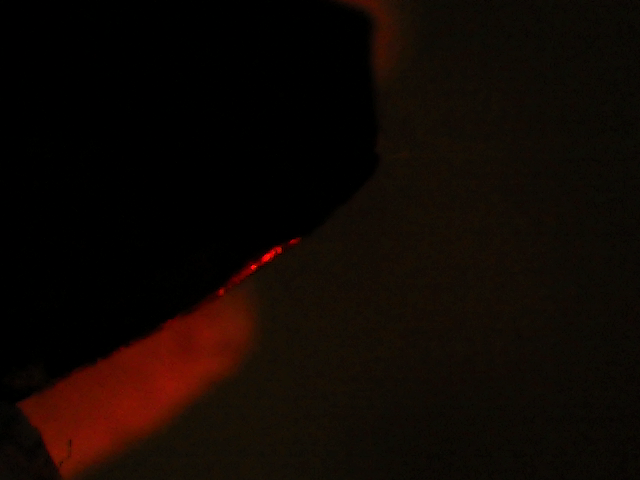
\includegraphics[width=3.125000in, keepaspectratio=true]{./fig/Vision/Dataset/automated_datasets/1_check_camera_position/2_camera_position_top/p3_l6.png}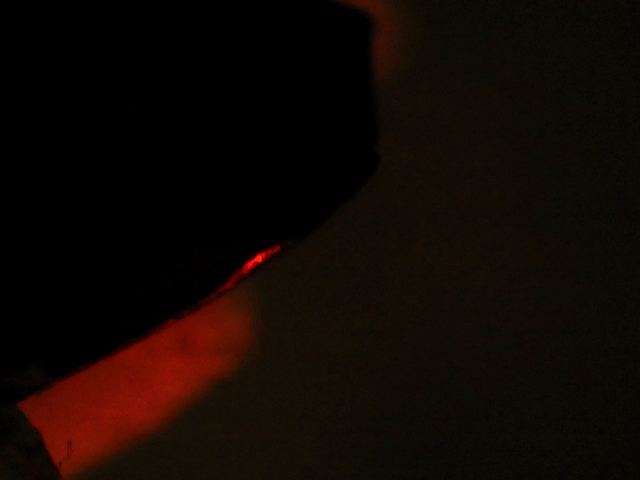
\includegraphics[width=3.125000in, keepaspectratio=true]{./fig/Vision/Dataset/automated_datasets/1_check_camera_position/2_camera_position_top/p3_l7.png}

On this data we can see the leds going up on the insert wear area. Which is what we tried to obtain. Now the leds are mapped to specific positions on the inserts and the amount of leds that need to be turned on for taking pictures can be reduced so no extra time is wasted. 




		\section{2 created datasets}

Created vrijdag 04 december 2020



The full datasets will be discussed in this page where firstly the dataset is documented and after that the tests that lead to this dataset are discussed.



\subsection{Birthday dataset}

Created a dataset on 27/11/2020 with a part of the given inserts for every possible color and led setting where pictures are taken from two separate led strips and every led one after another. This is done for white, red, green and blue colors. 

Done for batch 1 to 11





\subsection{spaghetti dataset}


		\section{1 Birthday dataset}

Created woensdag 02 december 2020





On November 27th a new dataset is created where for every plate 91 pictures are taken. 



The next pictures are available for the dataset:

\begin{itemize}
\item 1 picture with all leds on white
\item 30 pictures with red lighting; 15 of led strip A and 15 of led strip B
\item 30 pictures with blue lighting; 15 of led strip A and 15 of led strip B
\item 30 pictures with green lighting; 15 of led strip A and 15 of led strip B
\end{itemize}


The brightness is set to 80\% for all lights to make sure to not clip against the top values.



The dataset consists of 120*91 photos of 60 inserts with 120 worn sides. After 120 the quality was evaluated and the red, green and blue colors didn't seem to add more information to the pictures. 



In this dataset, there are some pictures unusable. As some worn areas are not even in the frame. Some to the left side and some to the right side. The placement of the wheel which holds the plates wasn't checkt thoroughly.

Picture 1: batch 3 insert 10 the side without bullet is off to the right side 

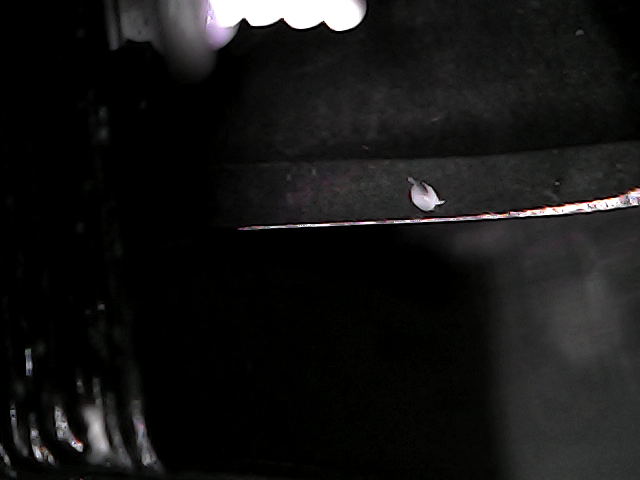
\includegraphics[width=4.166667in, keepaspectratio=true]{./fig/Vision/Dataset/automated_datasets/2_created_datasets/1_Birthday_dataset/b_003_p_010_l_000_nb.png}

picture 2: batch 3 insert 10 The side with bullet. Is far off to the left side.

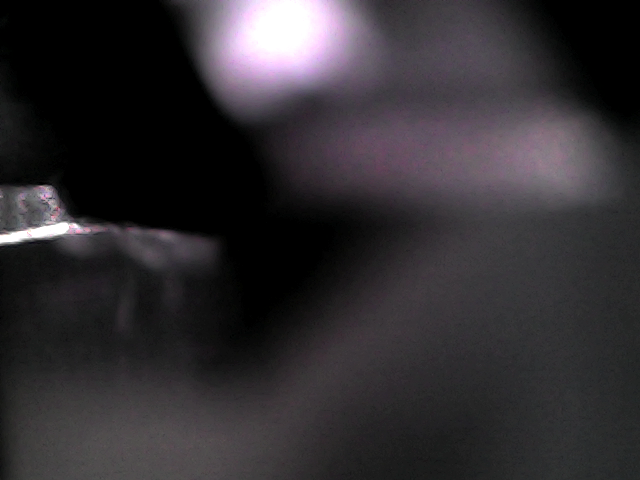
\includegraphics[width=4.166667in, keepaspectratio=true]{./fig/Vision/Dataset/automated_datasets/2_created_datasets/1_Birthday_dataset/b_003_p_010_l_000_b.png}



The setup for creating this dataset was as follows:

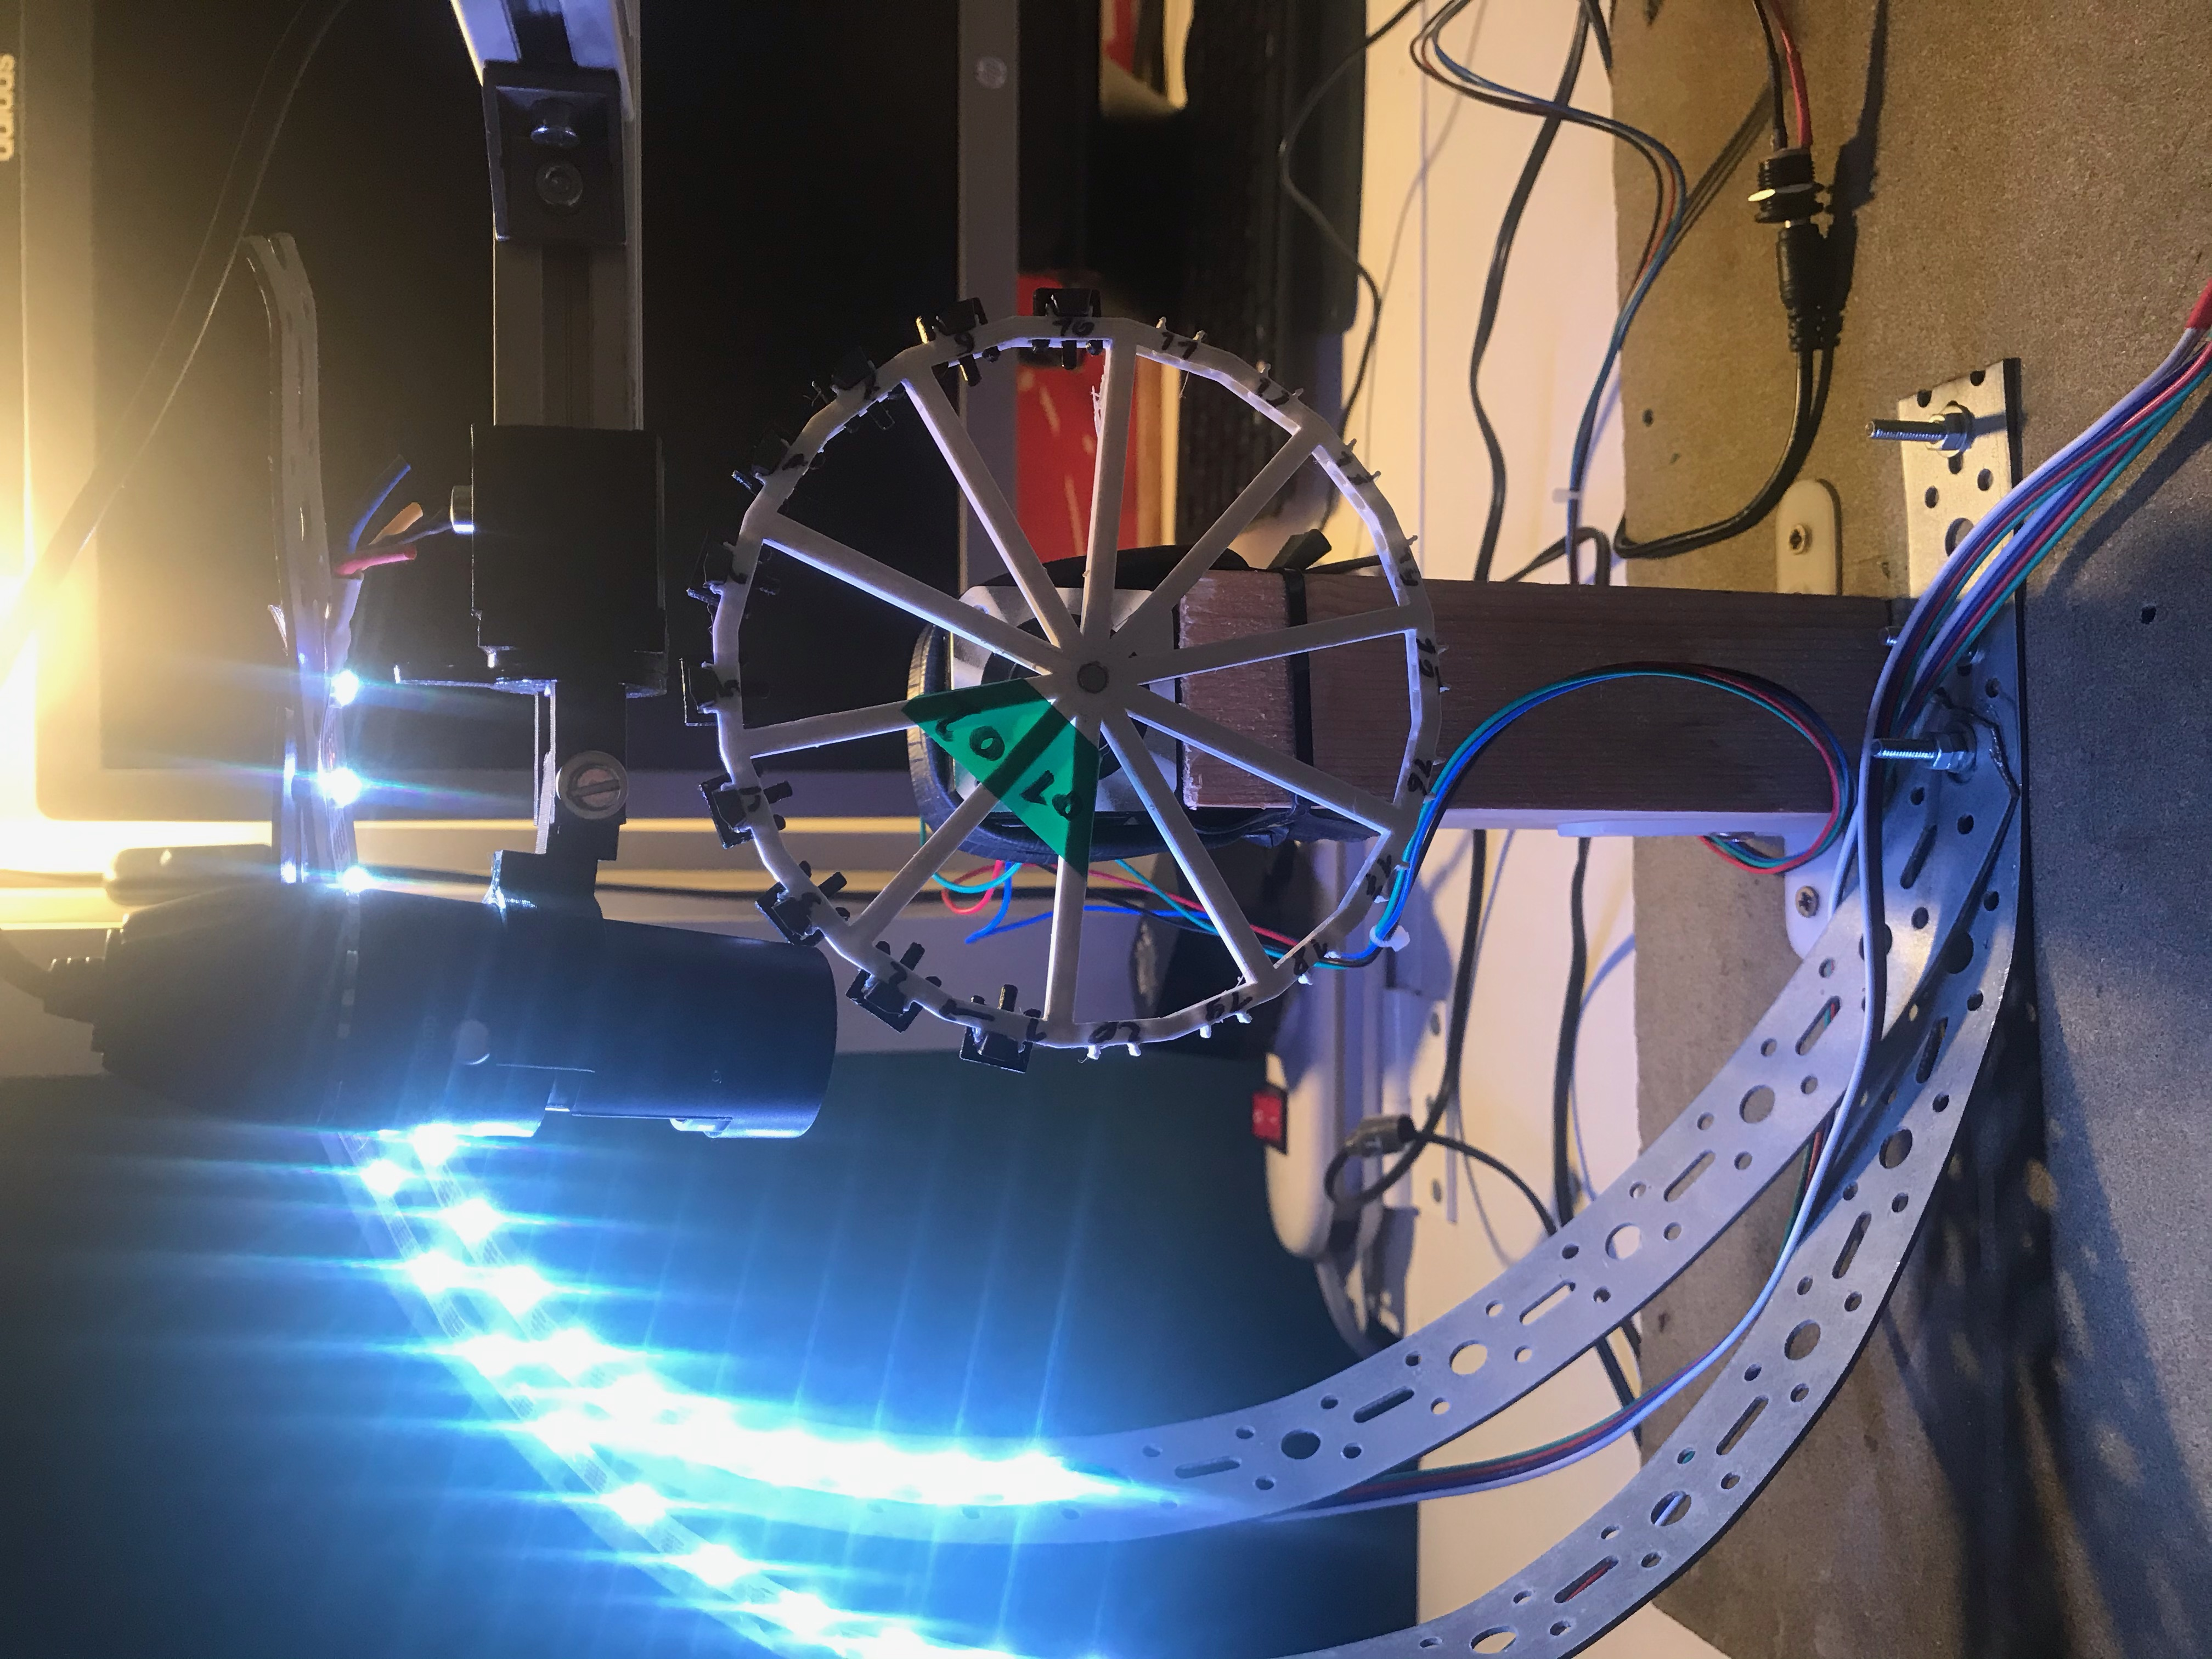
\includegraphics[width=4.166667in, keepaspectratio=true]{./fig/Vision/Dataset/automated_datasets/2_created_datasets/1_Birthday_dataset/IMG_9282.jpeg}

Here two ledstrips where mounted and pointed at the photographed insert. The inserts where attached to the wheel with black clips 3D printed with PETG. This was shosen above white clips to lower the light reflections into the camera lens. This was a problem in previous setups. 

Also a sturdy camera mount was fabricated out off metal profiles and 3D printed parts to get better notice of the placement of the camera opposed to the insert. 

The image taking process took about 1 minute per batch because of the amount of pictures taken. Since time was limited and the setup wasn't yet perfect we decided to only run 60 inserts through it. These where from batches 1 to 11. 

Sample pictures of this dataset can be found underneath. 

For every led one picture is taken. These images can be put together to create images on a full spectrum of leds and take out the best conditions. 

This can be done by inserting the images as different channels in the model.



The next pictures are from batch 3 insert 5 with led 6 turned on for both led strips and four colors.


\includegraphics[width=3.125000in, keepaspectratio=true]{./fig/Vision/Dataset/automated_datasets/2_created_datasets/1_Birthday_dataset/b_003_p_005_b_l_006_blue_A.png}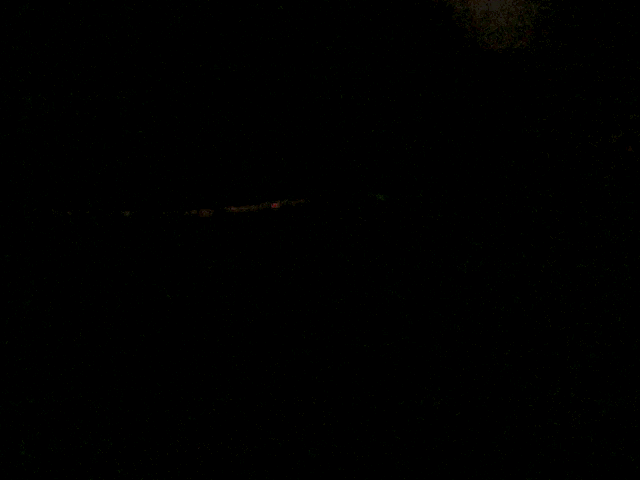
\includegraphics[width=3.125000in, keepaspectratio=true]{./fig/Vision/Dataset/automated_datasets/2_created_datasets/1_Birthday_dataset/b_003_p_005_b_l_006_red_A.png}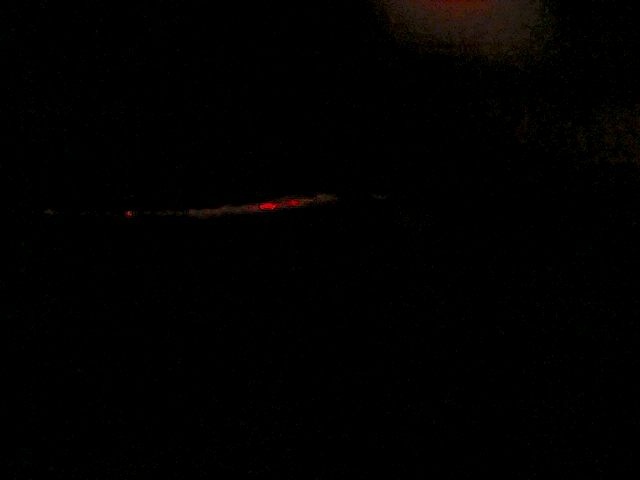
\includegraphics[width=3.125000in, keepaspectratio=true]{./fig/Vision/Dataset/automated_datasets/2_created_datasets/1_Birthday_dataset/b_003_p_005_b_l_006_red_B.png}
\includegraphics[width=3.125000in, keepaspectratio=true]{./fig/Vision/Dataset/automated_datasets/2_created_datasets/1_Birthday_dataset/b_003_p_005_b_l_006_green_A.png}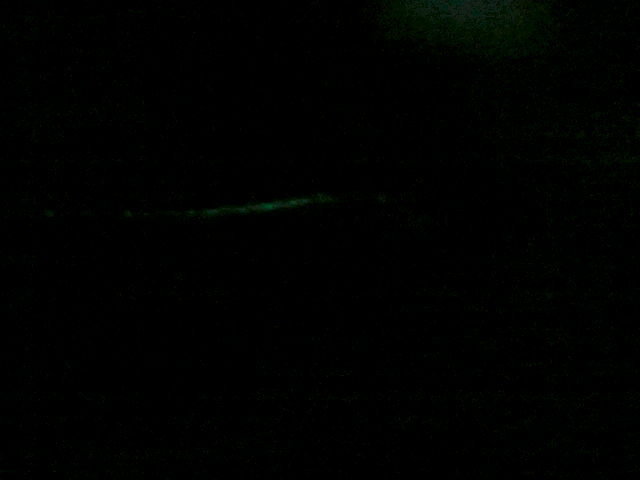
\includegraphics[width=3.125000in, keepaspectratio=true]{./fig/Vision/Dataset/automated_datasets/2_created_datasets/1_Birthday_dataset/b_003_p_005_b_l_006_green_B.png}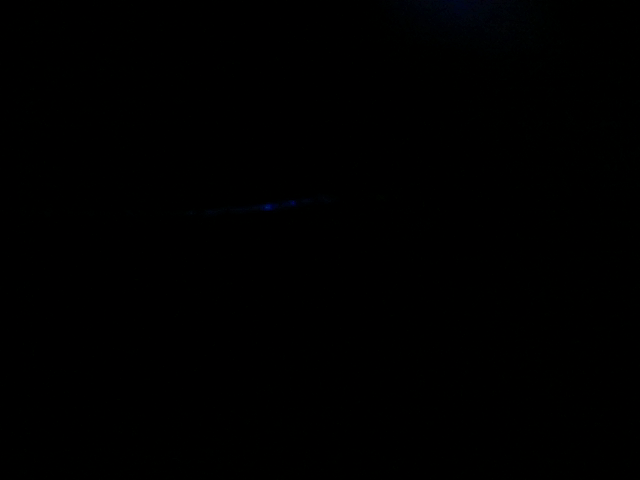
\includegraphics[width=3.125000in, keepaspectratio=true]{./fig/Vision/Dataset/automated_datasets/2_created_datasets/1_Birthday_dataset/b_003_p_005_b_l_006_blue_B.png}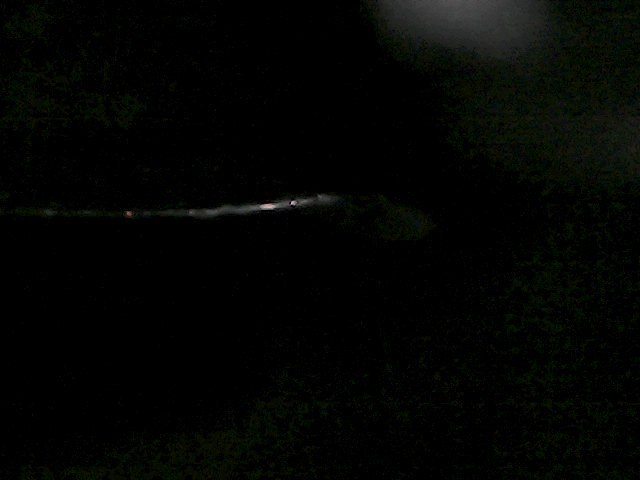
\includegraphics[width=3.125000in, keepaspectratio=true]{./fig/Vision/Dataset/automated_datasets/2_created_datasets/1_Birthday_dataset/b_003_p_005_b_l_006_white_B.png}
\includegraphics[width=3.125000in, keepaspectratio=true]{./fig/Vision/Dataset/automated_datasets/2_created_datasets/1_Birthday_dataset/b_003_p_005_b_l_006_white_A.png}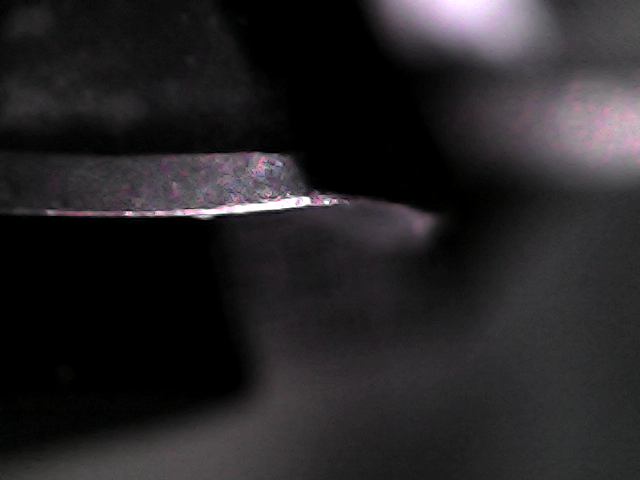
\includegraphics[width=3.125000in, keepaspectratio=true]{./fig/Vision/Dataset/automated_datasets/2_created_datasets/1_Birthday_dataset/b_003_p_005_l_000_b.png}

On these pictures we can see only red and white are visible and the B led strip wasn't visible. For this purpose the color of the wheel is changed to Black for less reflections. In the next dataset only white and red will be used for lighting. 



\subsection{Code}

The code used to process this data can be found in 


		\section{conducted tests before creation}

Created vrijdag 27 november 2020



Getting first full dataset with images of all plates



\subsection{First test}

first pictures formatted with 

b\_xxx\_p\_xxx\_l\_xxx.png

	-\textgreater{} these images where from last time checking some setups
	
	



\subsection{Second test}

formatting 

next pictures without changing for different led strips

b\_xxx\_p\_xxx\_color\_l\_xxx.png



\subsection{Third test}

formatting

pictures with full experiments on lid lighting

b\_xxx\_p\_xxx\_color\_strip\_l\_xxx\_bullet.png

a video is taken here 

Here we can see a difference with or without light in the room



reformatted last images to be able to see difference between different leds, bet setup and runs are the same

b\_xxx\_p\_xxx\_bullet\_l\_xxx\_color\_strip.png





possibly 3 and 4 no bullet wrong 

rest went okay just check the batches 3 and 4



\subsection{Birthday dataset}

batch 3 plate 7 no bullet:  had restants of 3D print plastic on worn area

batch 3 plate 8 no bullet:  is a bit off picture

from here in batch 3 plates go out of sight for no bullet side. 



bullet side is going the other way out of sight for batch 3 

batch four starts of with bad pictures (also b on the left out of sight and nb on the right side out of sight



from batch 4 plate 7 it is okay again



batch 5 plate 6 no bullet lighting not good

batch 5 plate 6 bullet has string from 3D printing on wear area



batch 11 plate 5 bullet had hair on wear area


		\section{2 Spaghetti dataset}

Created vrijdag 04 december 2020



After the Birthday dataset a new dataset was created using the things learned from that. Now the amount of leds driven is reduced to 5 leds. Where led 6 to 11 is used to lighten the inserts. 

only the colors white and red are used for this dataset. This was discussed thad the red color could have an influence on the reflection of the carbide of which the inserts are made see light reflection.



\subsection{Dataset explanation}

For every insert, two pictures are taken. One with leds 6 to 11 on red and one with these leds white. This was experimentally found to be the best setting for reflecting the light off the worn area and into the camera. 

Turning on a led to much on the upper bounary will lighten the side of the insert which isn't of much use in this paper. Turining on a led to much on the bottom boundary makes the background very bright which supports unnessesary information.



The images are separated in a folder for every insert named with batch number and insert number:

batch\_aaa\_plate\_bbb where aaa is the batch number and bbb is the insert number.

Images are named with their settings, batch number and insert number:

b\_aaa\_p\_bbb\_l\_006-011\_color\_bullet.png 

where 

\begin{itemize}
\item aaa is the batch number; 
\item bbb is the plate number, 
\item 006-011 are the leds that turned on at the same time; 
\item color is the color: red or white
\item bullet is the appearance of a bullet on the side of the inset and has values of b for bullet or nb for no bullet.
\end{itemize}


The dataset inserts consisted of a few different types and coatings. 



\subsection{Setup}

The setup used is exactly the same as on the Birthday dataset where the camera is positioned as much to the top as possible. This can be seen on the picture:

Here we can see the led strips are a little bit twisted and are positioned very close to each other. This made the reflection better and should result in beter outcome of the algorithm.



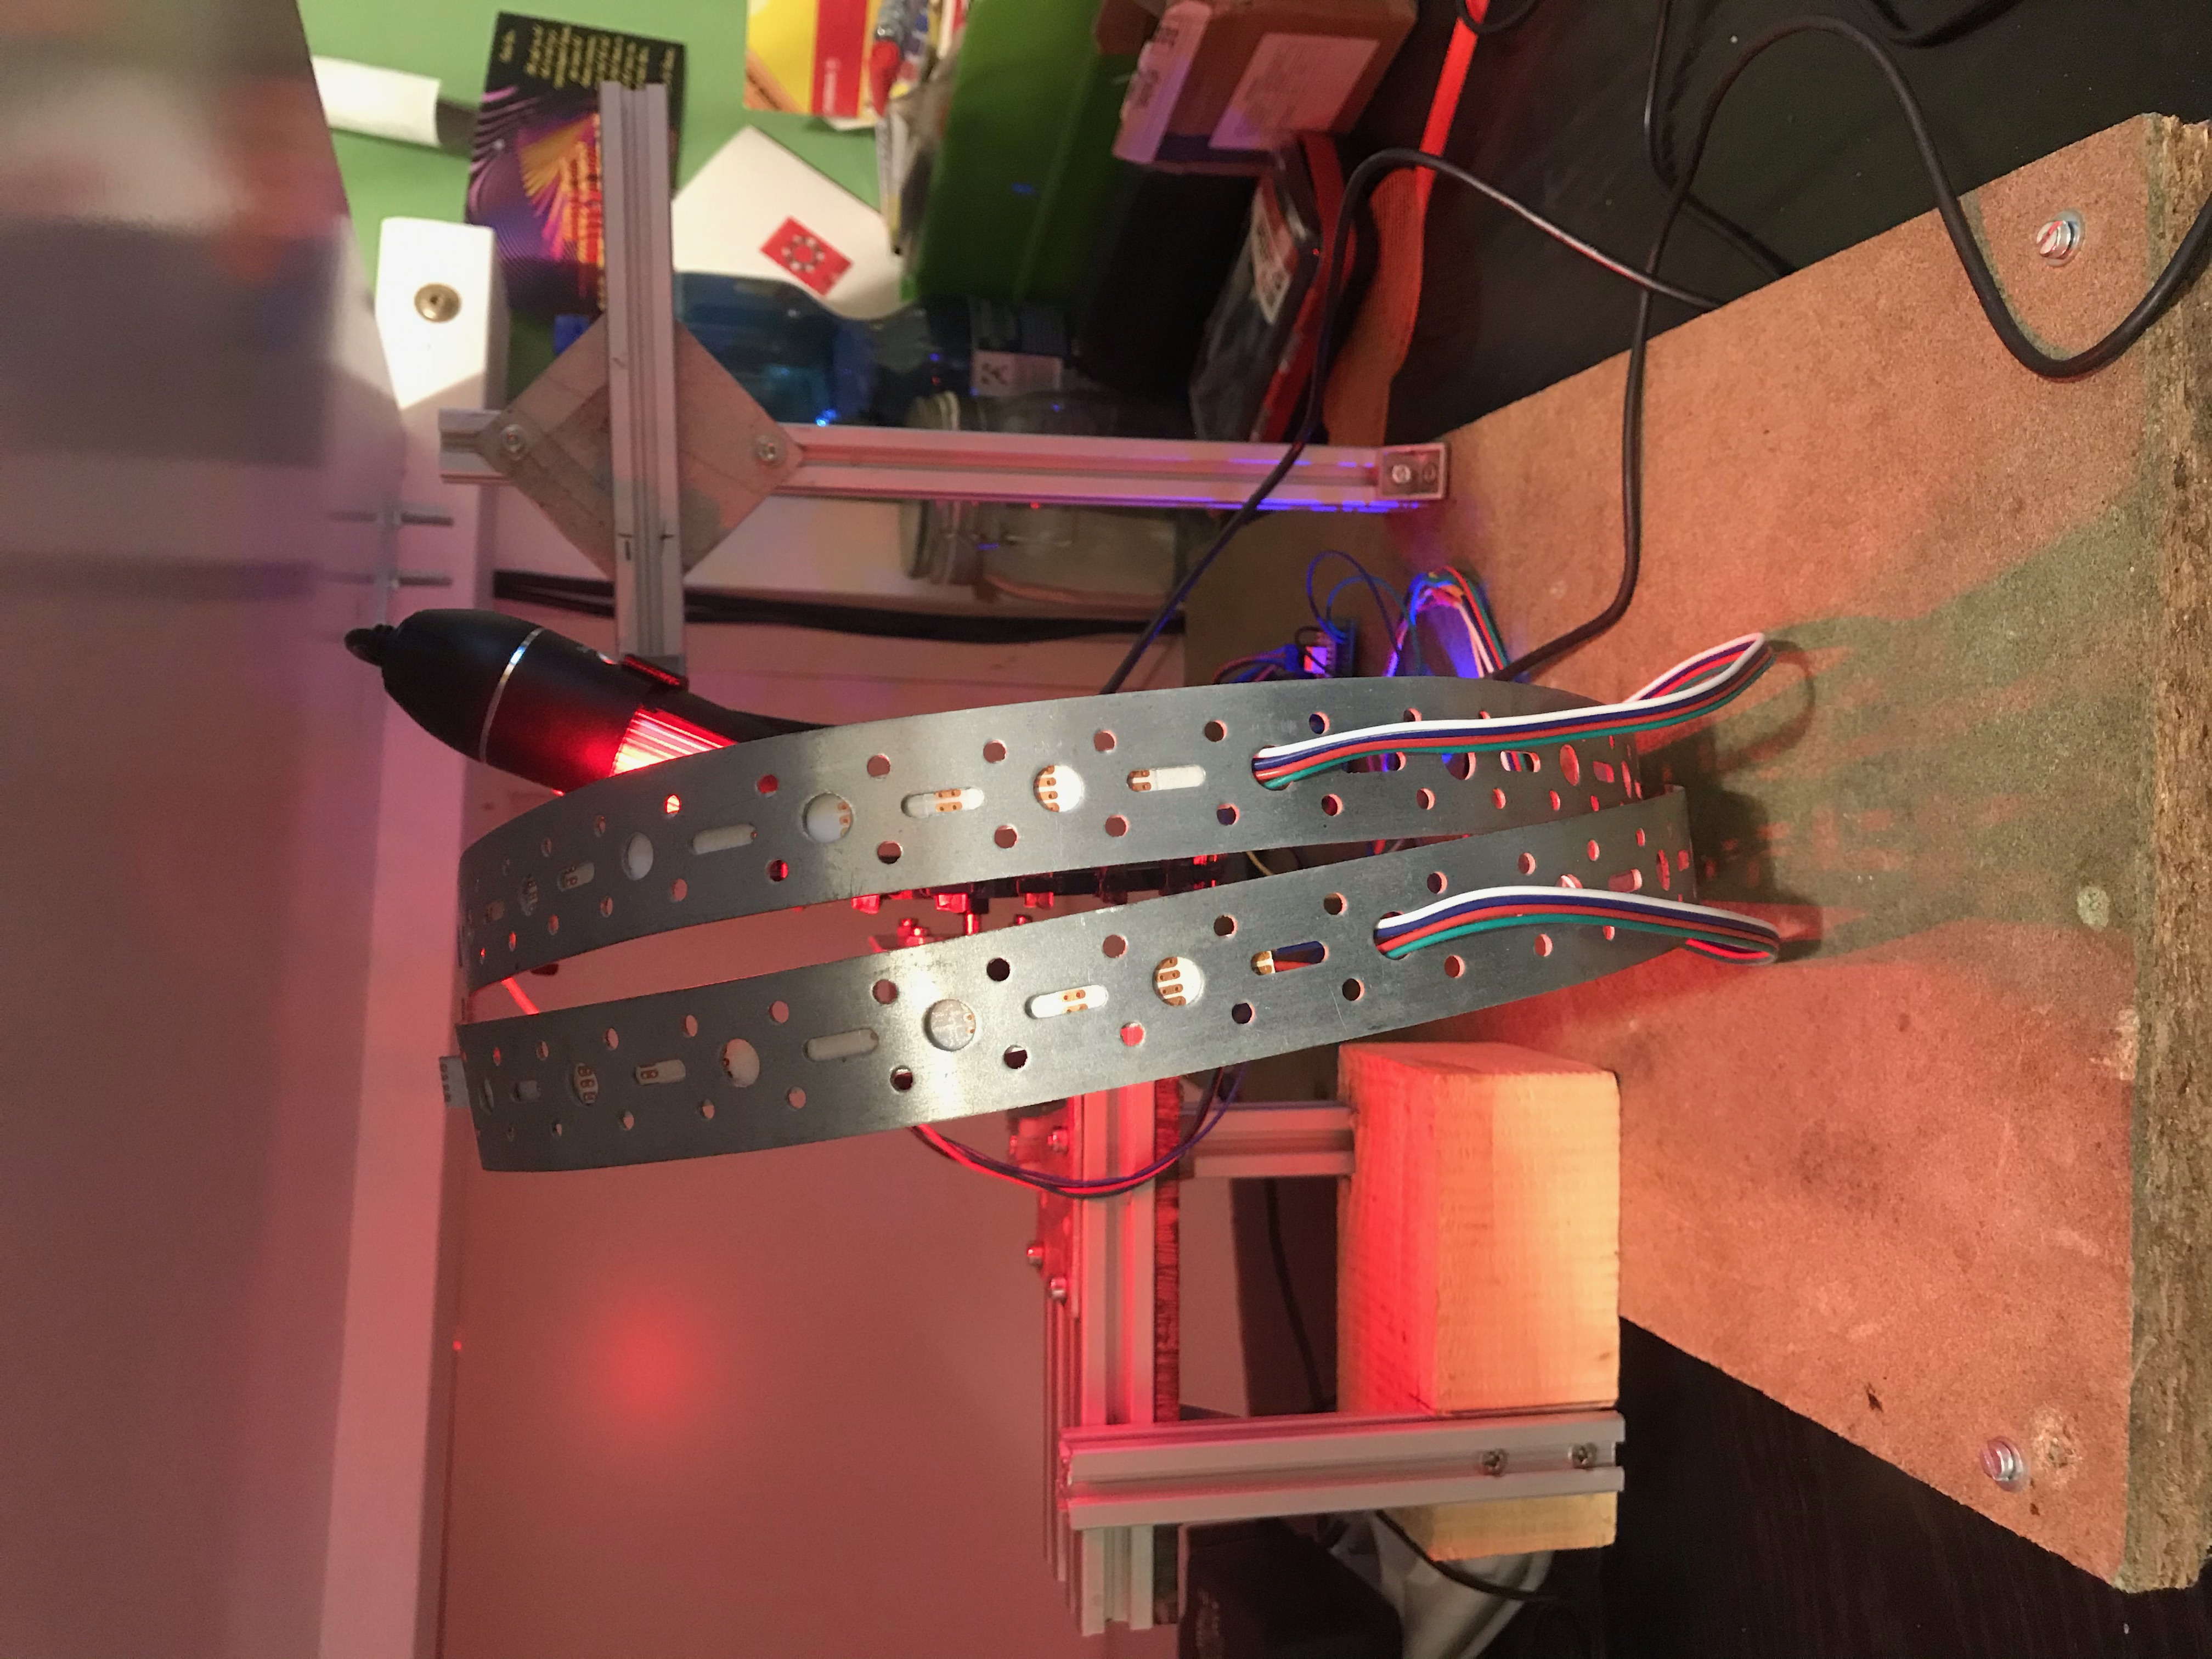
\includegraphics[width=4.166667in, keepaspectratio=true]{./fig/Vision/Dataset/automated_datasets/2_created_datasets/2_Spaghetti_dataset/IMG_9295.jpeg}



The camera angle is kept the same a little to the top and very close to the inserts as seen on the next picture:

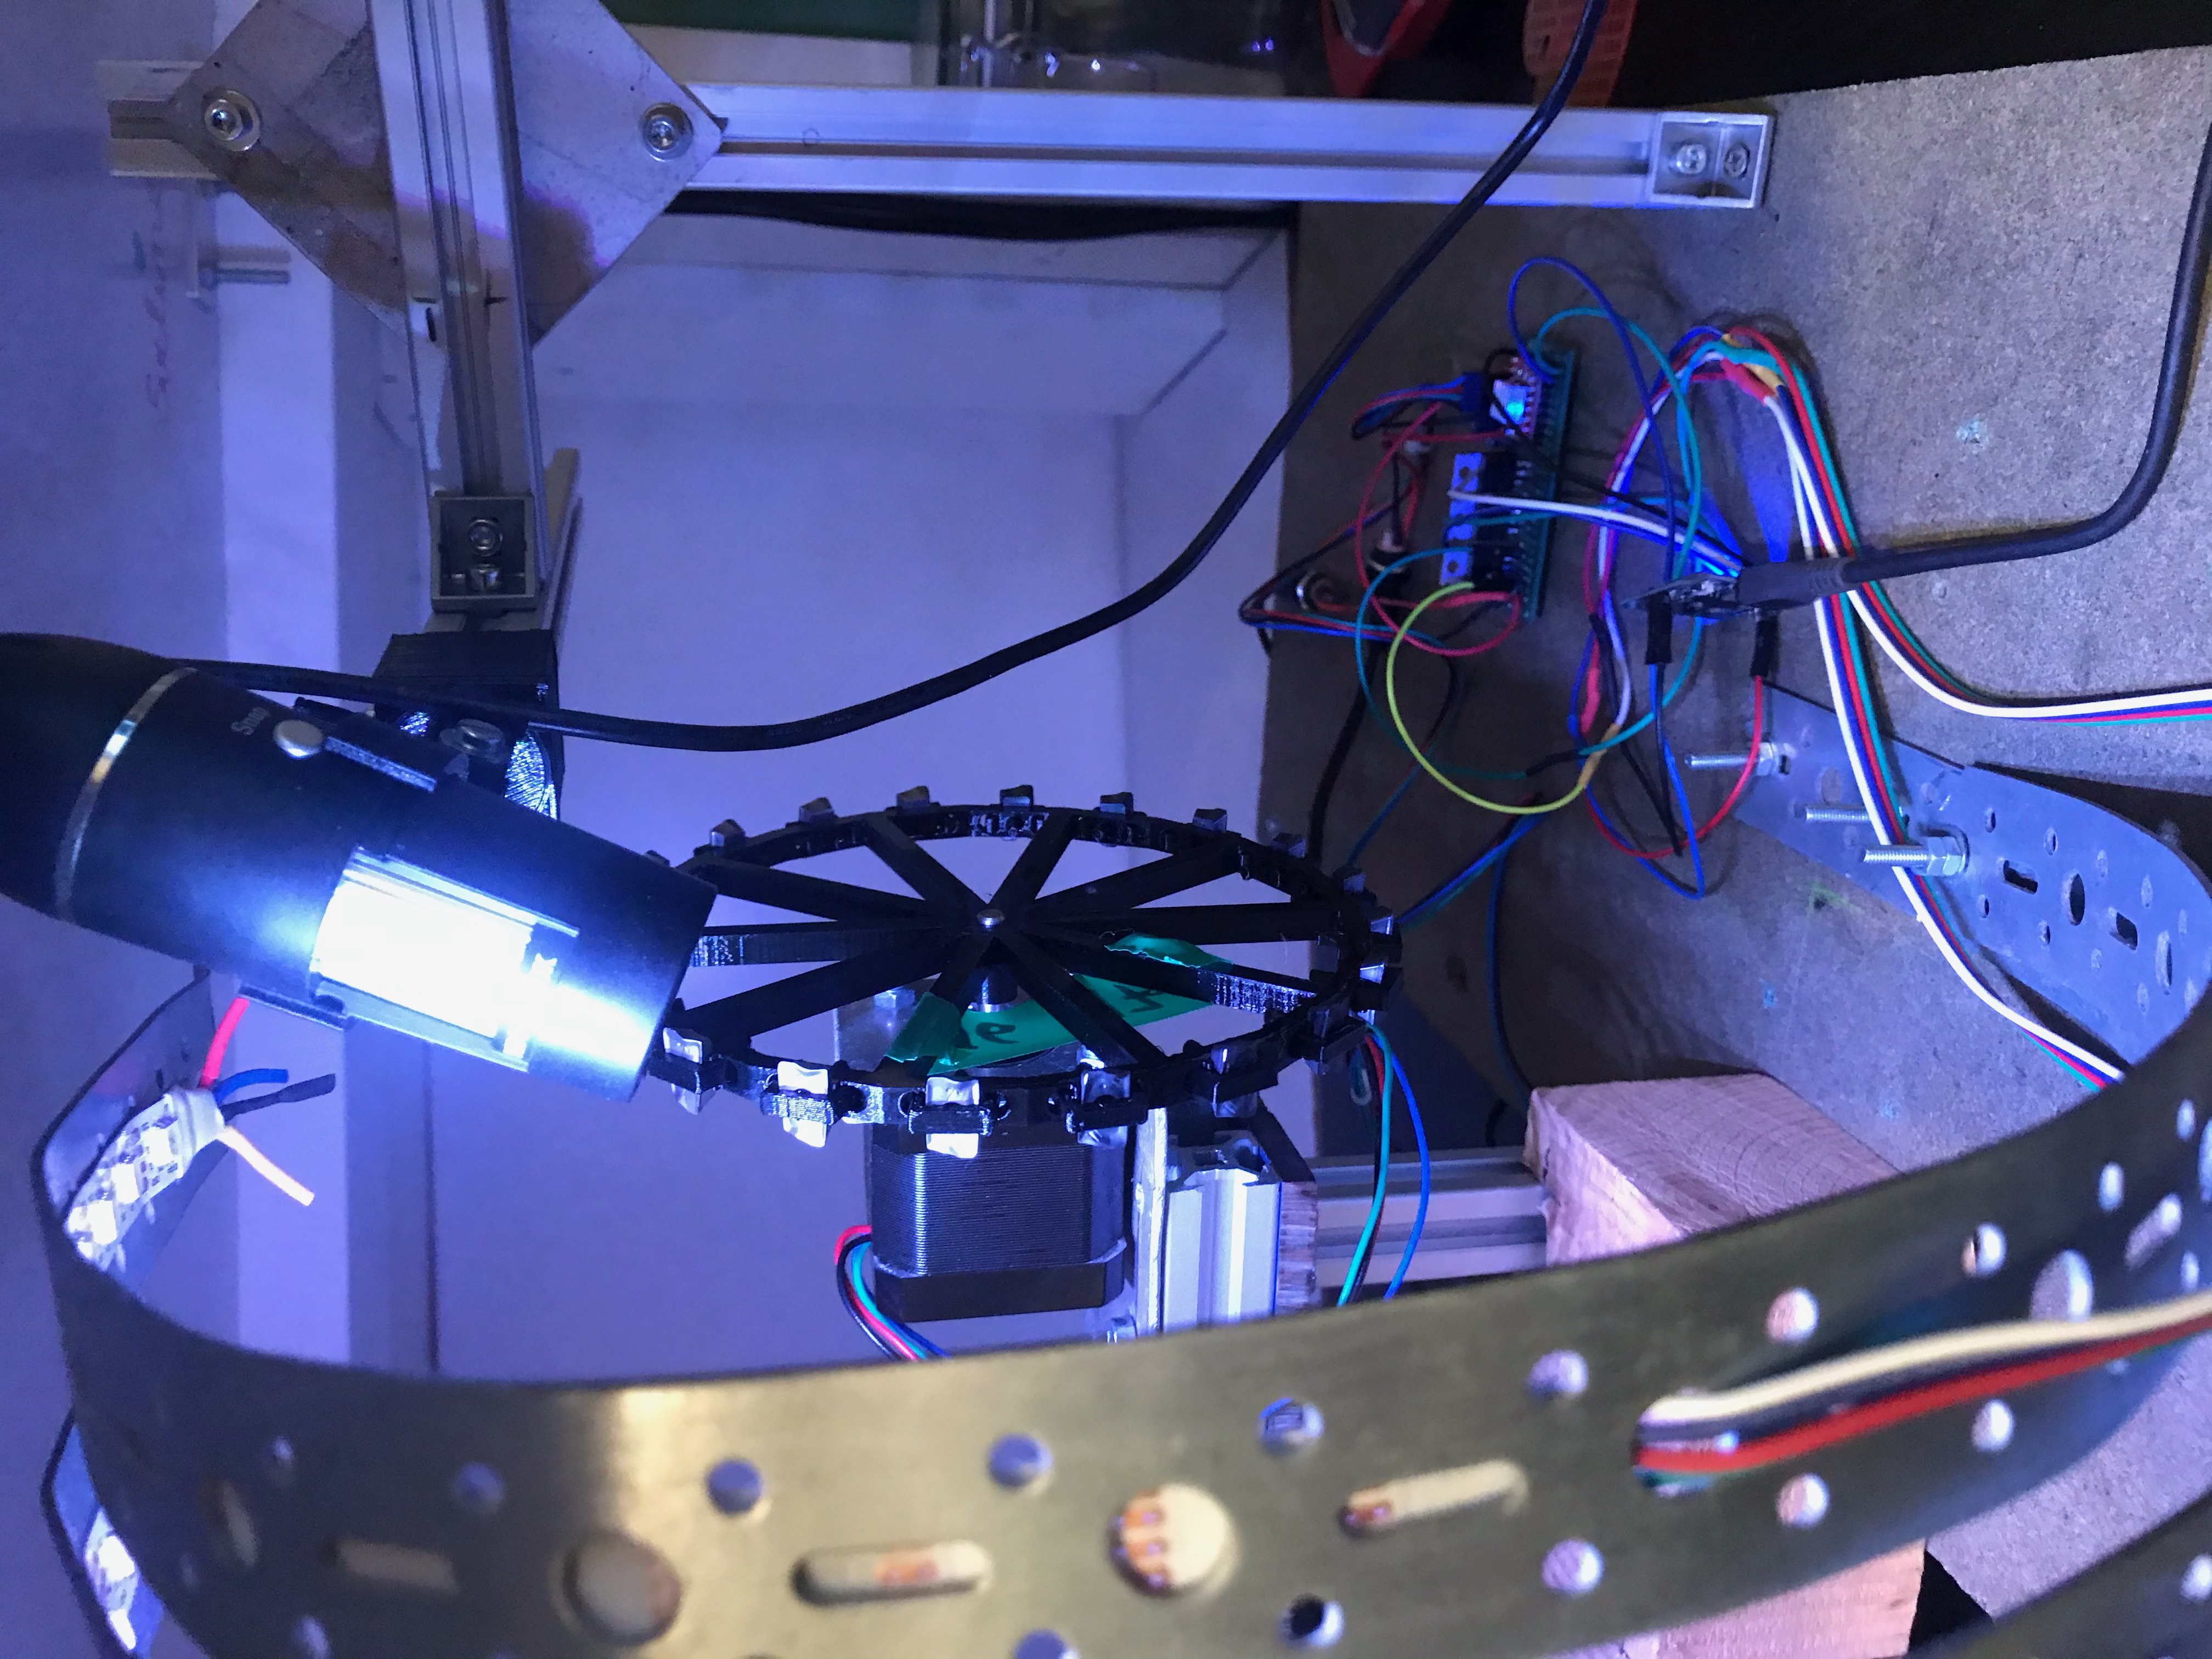
\includegraphics[width=4.166667in, keepaspectratio=true]{./fig/Vision/Dataset/automated_datasets/2_created_datasets/2_Spaghetti_dataset/IMG_9296.jpeg}



Through the whole dataset the direct light coming from other sources eg. the light of the room was blocked to have full control of the lighting conditions.



\subsection{Results}

Underneath are some pictures of good examples in the dataset.



Underneath are two pictures of batch 3 insert 6. These where lid with red light on the left and white light on the right. Here is a nice wear shown and lighted. However if we zoom in to the picture the top part of the wear is not lighted that well. We can also see a white piece of the insert holder on the image which is providing som extra difficulties. The discussion of these difficulties will be bespoken in vision algorithm.

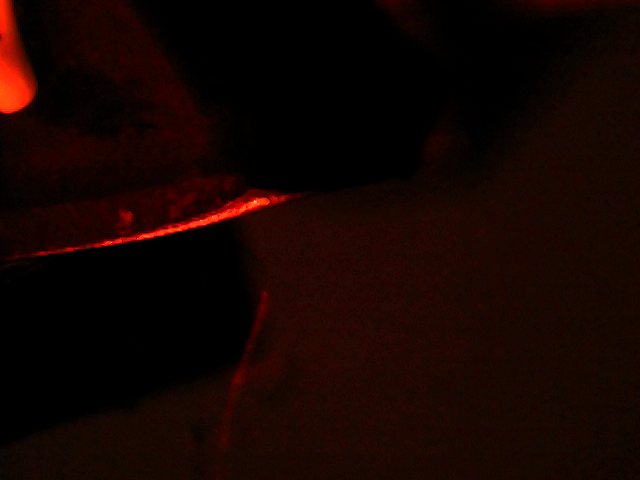
\includegraphics[width=3.125000in, keepaspectratio=true]{./fig/Vision/Dataset/automated_datasets/2_created_datasets/2_Spaghetti_dataset/b_003_p_006_l_006-011_red_nb.png}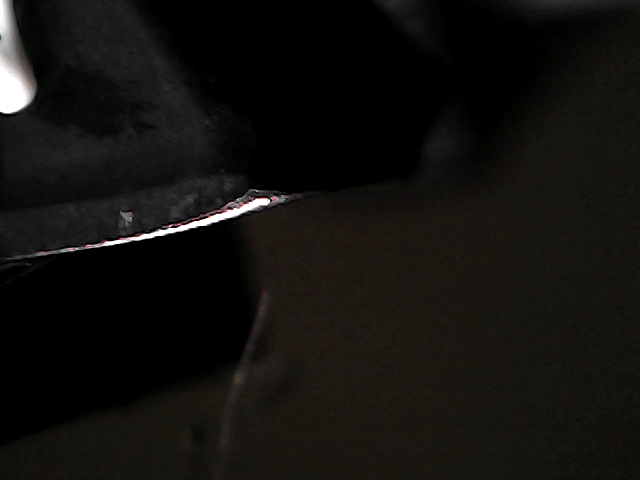
\includegraphics[width=3.125000in, keepaspectratio=true]{./fig/Vision/Dataset/automated_datasets/2_created_datasets/2_Spaghetti_dataset/b_003_p_006_l_006-011_white_nb.png}



Some pictures aren't sharp like the one shown next.

like batch 5 insert 5 withoud bullet.

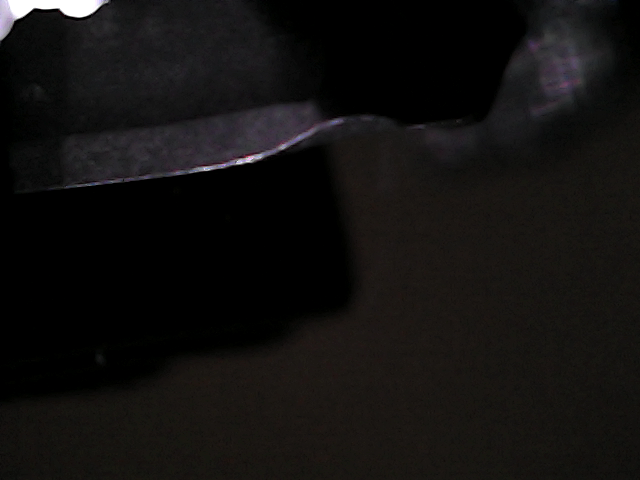
\includegraphics[width=3.125000in, keepaspectratio=true]{./fig/Vision/Dataset/automated_datasets/2_created_datasets/2_Spaghetti_dataset/b_005_p_005_l_006-011_white_nb.png}



\paragraph{Different insert types}

First type are the grey inserts with very visible wear. These are seen in batches 1 to 5 consistently. This type will be called grey inserts.

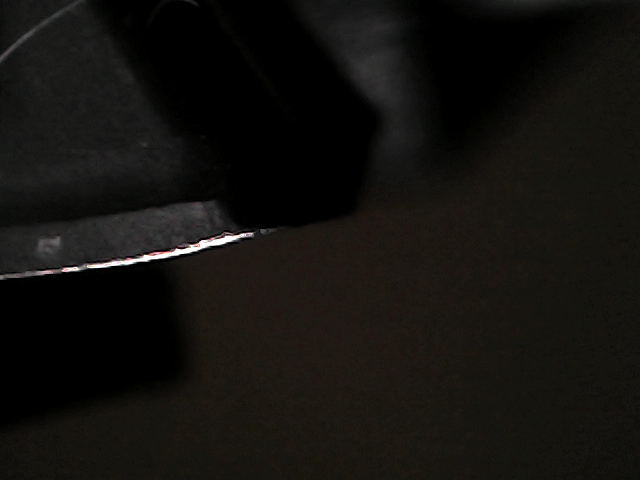
\includegraphics[width=3.125000in, keepaspectratio=true]{./fig/Vision/Dataset/automated_datasets/2_created_datasets/2_Spaghetti_dataset/gray_b_003_p_004_l_006-011_white_nb.png}



Than there are other inserts in batch 11 which are also grey but have a different shape on the cutting part. These will be called rounded grey inserts.

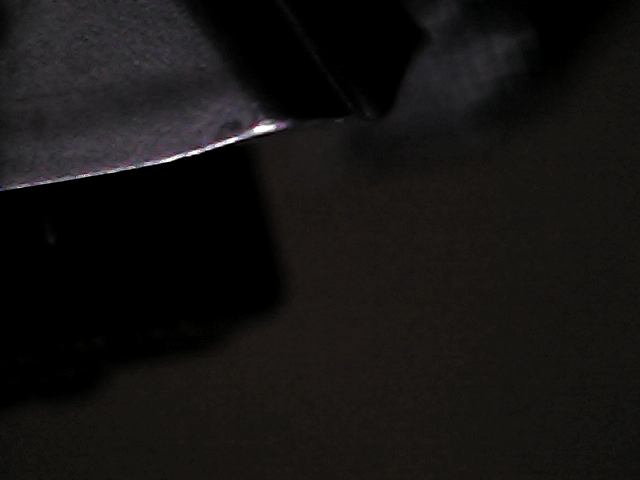
\includegraphics[width=3.125000in, keepaspectratio=true]{./fig/Vision/Dataset/automated_datasets/2_created_datasets/2_Spaghetti_dataset/rounded_grey_b_011_p_008_l_006-011_white_nb.png}

In batch 12 and 13 there are the same shape of inserts but with a black coating which results in way darker pictures as seen here on batch 13 insert 2 no bullet. These inserts are the rounded black inserts.

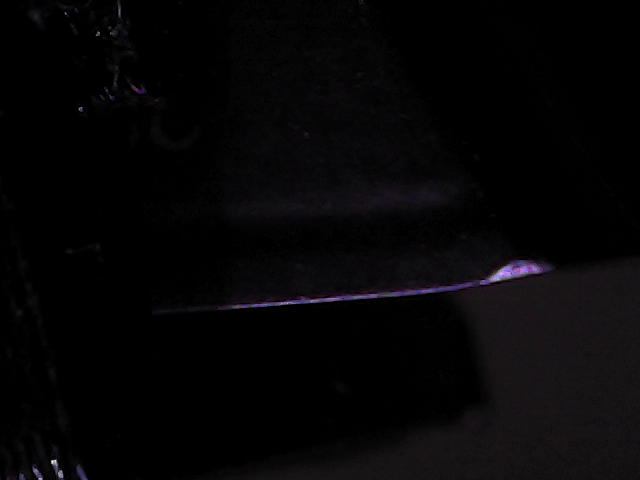
\includegraphics[width=3.125000in, keepaspectratio=true]{./fig/Vision/Dataset/automated_datasets/2_created_datasets/2_Spaghetti_dataset/rounded_black_b_013_p_002_l_006-011_white_nb.png}



The next type are copper colored inserts with the rounded shape. Seen in batch 14 insert 5 no bullet.

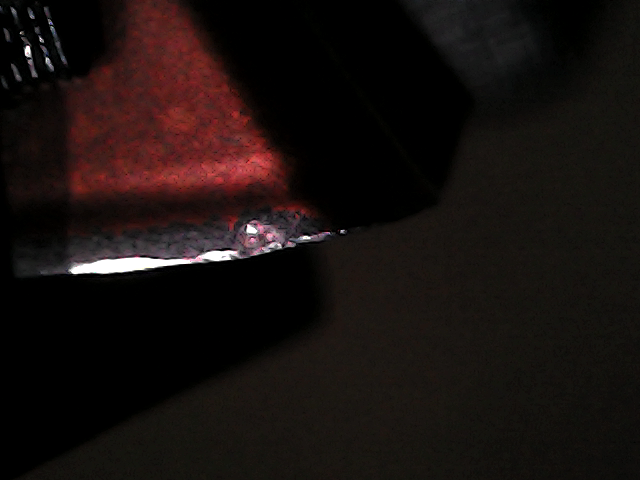
\includegraphics[width=3.125000in, keepaspectratio=true]{./fig/Vision/Dataset/automated_datasets/2_created_datasets/2_Spaghetti_dataset/rounded_copper_b_014_p_005_l_006-011_white_nb.png}



Than we have inserts with a gold coating and hooked shape. For batch 15 insert 6 no bullet that gives the next picture:

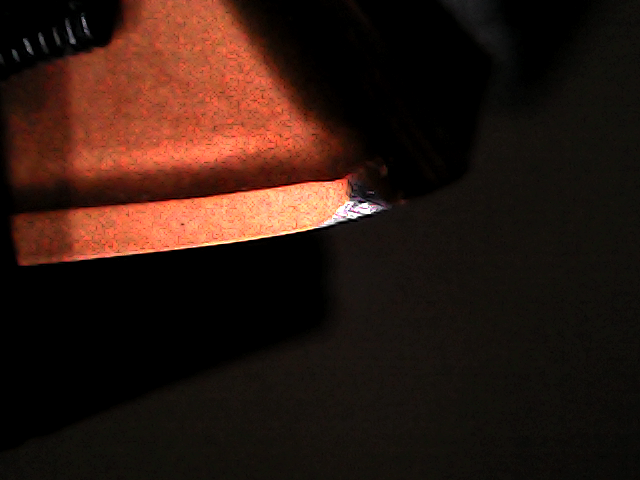
\includegraphics[width=3.125000in, keepaspectratio=true]{./fig/Vision/Dataset/automated_datasets/2_created_datasets/2_Spaghetti_dataset/rounded_gold_b_015_p_006_l_006-011_white_nb.png}

\section{camera position}

Created woensdag 11 november 2020



1st test was with a camera position more to the side of the cutting plates. This resulted in a bad reflection angle since the light came from the wrong side. Documentation of this set is in automated datasets:1 check camera position:1 camera position side


		\section{handmade datasets}

Created vrijdag 04 december 2020




		\section{initial dataset}

Created vrijdag 13 november 2020



\subsection{Form}

The dataset given where taken with a microscopic camera at Sirris. These images were in good lighting conditions for the measurement, but had a lot of extra "unwanted" features on it. The background was very like the wear and the rest of the tool insert. 

Every insert that was measured had a little mark on one side to mark the a and b. Sadly the information about what the marker meant is lost. To find the corresponding values, the inserts where once again put through a microscopic camera and the new pictures where compared against the old ones. 



While again checking the inserts out, a new dataset is created since this didn't ask much more time. During this proces there is also a new way of separating the sides of the inserts. There is a bullet at one side on every insert. This is an easy way to recognise a side and wont dissapear like the marker line. 







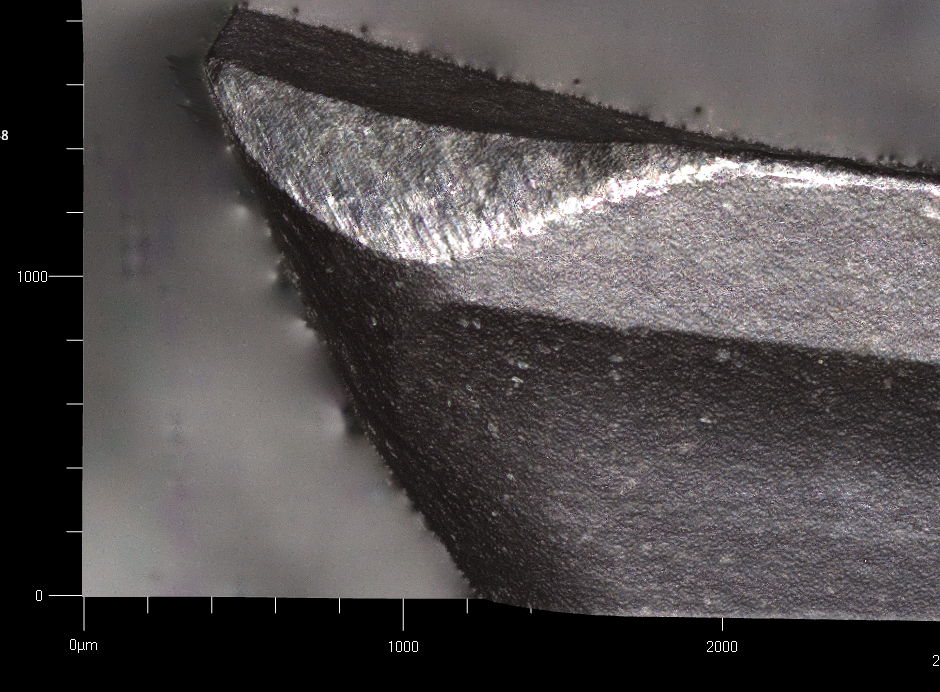
\includegraphics[width=3.125000in, keepaspectratio=true]{./fig/Vision/Dataset/handmade_datasets/initial_dataset/initial dataset pictuer.PNG}




		\section{Second handmade dataset}

Created vrijdag 13 november 2020



A second handmade dataset is made to compare with the first dataset and get to know what the stripes mean on the first dataset which was used to measure the wear.



The next setup is used:

The light came primarely from the camera itself which was set in the first brightness setting. 

The camera was located at a distance of 2cm between the housing and the measured point on the insert. The housing starts at the black part; not the plexi glass protector. 

During the making of this dataset the inserts where labeled with bullet or no bullet. This was not setup this way in the first place; instead there was a marker line on the insert. This marker line is also noted in the labels of the dataset.

An "s" means it is with a marker line. A

\begin{tabular}{ |l|l| }
\hline
 symbol & explanation \tabularnewline
\hline
\hline
 s & side with marker line \tabularnewline
\hline
 n & side without marker line \tabularnewline
\hline
 batch number & number specified on the box in which the inserts are kept \tabularnewline
\hline
 plate number & number specified inside the box; this goes from 1 to 10 per batch \tabularnewline
\hline
\end{tabular}


The naming of the dataset is the following

b\_\textless{}batch number\textgreater{}\_p\_\textless{}plate number\textgreater{}\_\textless{}identifier of side\textgreater{}

After looking at the pictures of the datasets it can be confirmed that the 'b' side of the inserts is the side with the mark on. 



This can be seen on the folowing two pictures whis correspond. The first one is from the first dataset, the second from the second dataset.

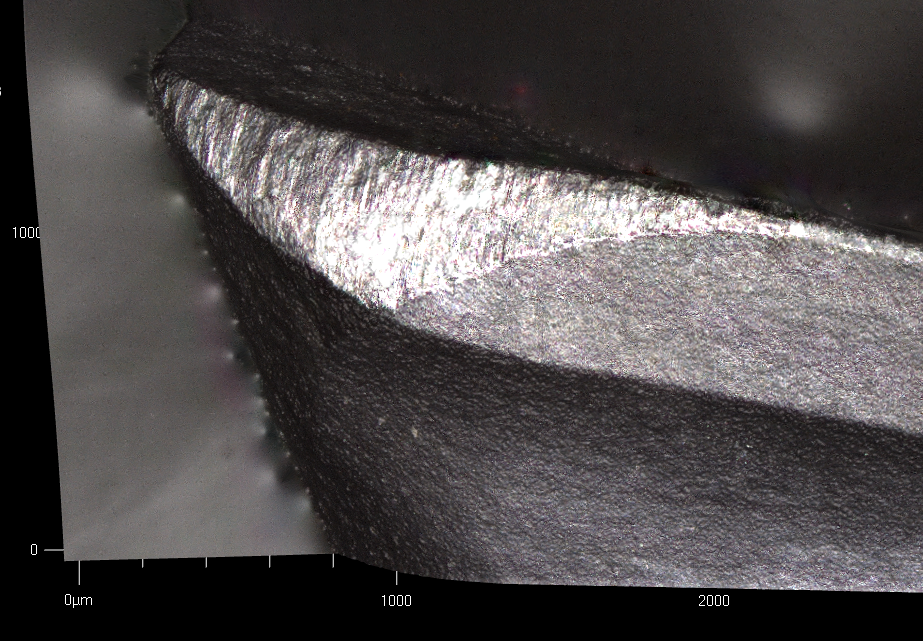
\includegraphics[height=2.083333in, keepaspectratio=true]{./fig/Vision/Dataset/handmade_datasets/Second_handmade_dataset/t50b-img.PNG}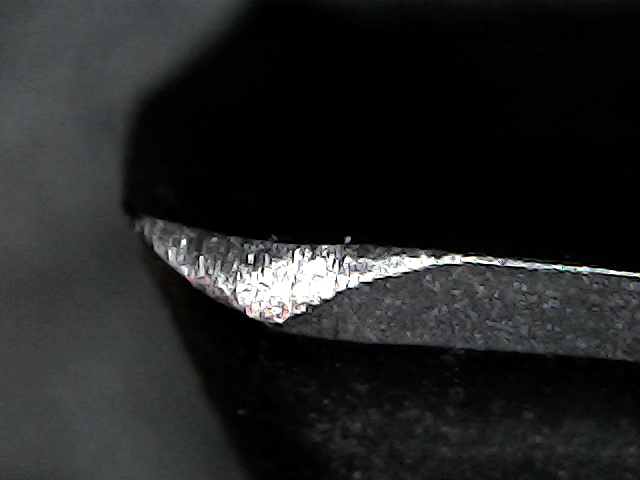
\includegraphics[height=2.083333in, keepaspectratio=true]{./fig/Vision/Dataset/handmade_datasets/Second_handmade_dataset/b_005_p_010_s.jpg}


		\section{second initial dataset}

Created vrijdag 04 december 2020



With the second number of inserts (batch 11 to 19) another dataset was created for measurement.

Since the photo's where labeled with two inserts at a time; the images taken where not relevant for the data processing and were not saved



The distance for these inserts is measured between the line connecting the two highest points visible on the insert and the outer most point of the wear area.

\section{Google Colab}
\section{Test Camera Setup}

Created woensdag 04 november 2020



To test the camera setup, a binary classification model is made. This model will tell with a treshold of 150 (200 the real treshold but 150 to warn before tool is worn out) wether a tool is good to work with or must be removed from the machine. 

This model should be trainable with as less images as possible, preferably 20 because that is the amount of pictures taken in one batch.





\subsection{Resnet18}

First we will try to implement SDD-Resnet18 to classify the few images in good or bad. 



\subsection{nception v3}

Than we will implement SDD-inception v3 



These described models should perform rather good without any transfer learning. 

After the first tests these results can be compared with a transfer learning model.





\subsection{All Networks}

For this all networks test, some networks where tested and an algorithm is created to make it possible to add more networks along the way


		\section{All Networks}

Created woensdag 02 december 2020




		\section{All Networks 1}

Created woensdag 02 december 2020



All networks 1 can be found \href{https://colab.research.google.com/drive/1bWt0DgypiYoOOgnSGjlmSdDo7elvJnH4}{here.}



\subsection{Network architectures}

This model is used to test different model architectures namely:

\begin{itemize}
\item Resnet18
\item Alexnet
\item VGG11\_bn
\item Squeezenet
\item Densenet
\end{itemize}


inception v3 didn't seem to work



These models are all relatively small and should provide quite good results for a small dataset. 

More on why the models should work can be found here



\subsection{Dataset}



This algorithm had the input of images from the Second handmade dataset which was devided into 3 classes based on their measured wear value. 

\begin{tabular}{ |l|l|l| }
\hline
 class & min value (micron) & max value (micron) \tabularnewline
\hline
\hline
 good & 0 & 130 \tabularnewline
\hline
 medium & 130 & 230 \tabularnewline
\hline
 bad & 230 & ∞ \tabularnewline
\hline
\end{tabular}










\subsection{Results}

Results of this notebook are available on wandb as \href{https://wandb.ai/dplars/pytorch-TWI_second_handmade?workspace=user-dplars}{pytorch-TWI\_second\_handmade}



Interesting results will be bespoken here;

Tests for different models: 

\begin{tabular}{ |l|l|l|l| }
\hline
 model name & test accuracy \% & validation accuracy\% & transfer learning \tabularnewline
\hline
\hline
 Alexnet & 100 & 90 & yes \tabularnewline
\hline
 VGG11\_bn & 89 & 85 & yes \tabularnewline
\hline
 Densenet & 89 & 85 & yes \tabularnewline
\hline
 Squeezenet & 89 & 85 & yes \tabularnewline
\hline
 Resnet18 & 89 & 90 & no \tabularnewline
\hline
\end{tabular}
										

An overview of the best runs for every model architecture. Since there are only nine test images; the test scores are set to a very high granularity. Further results of this test are to be found on wandb as \href{https://wandb.ai/dplars/pytorch-TWI_second_handmade/reports/Testing-on-first-handmade-dataset--VmlldzozNTE5NzM}{Testing on first handmade dataset}


		\section{All Networks 2}

Created vrijdag 04 december 2020



\subsection{Network architectures}

This model is used to test different model architectures namely:

\begin{itemize}
\item Resnet18
\item Alexnet
\item VGG11\_bn
\item Squeezenet
\item Densenet
\end{itemize}


inception v3 didn't seem to work



These models are all relatively small and should provide quite good results for a small dataset. 

More on why the models should work can be found here



\subsection{Dataset}



This algorithm had the input of images from the Second handmade dataset which was devided into 3 classes based on their measured wear value. 

\begin{tabular}{ |l|l|l| }
\hline
 class & min value (micron) & max value (micron) \tabularnewline
\hline
\hline
 good & 0 & 130 \tabularnewline
\hline
 medium & 130 & 230 \tabularnewline
\hline
 bad & 230 & ∞ \tabularnewline
\hline
\end{tabular}










\subsection{Results}

Results of this notebook are available on wandb as \href{https://wandb.ai/dplars/pytorch-TWI_second_handmade?workspace=user-dplars}{pytorch-TWI\_second\_handmade}



Interesting results will be bespoken here;

Tests for different models: 

\begin{tabular}{ |l|l|l|l| }
\hline
 model name & test accuracy \% & validation accuracy\% & transfer learning \tabularnewline
\hline
\hline
 Alexnet & 100 & 100 & yes \tabularnewline
\hline
 Resnet18 & 100 & 95 & no \tabularnewline
\hline
 Densenet & 100 & 85 & yes \tabularnewline
\hline
 Squeezenet & 100 & 85 & yes \tabularnewline
\hline
 VGG11\_bn & 100 & 90 & no \tabularnewline
\hline
\end{tabular}
										

An overview of the best runs for every model architecture. Since there are only nine test images; the test scores are set to a very high granularity. Further results of this test are to be found on wandb as \href{https://wandb.ai/dplars/pytorch-TWI_second_handmade/reports/Testing-on-first-handmade-dataset--VmlldzozNTE5NzM}{Testing on first handmade dataset}





Trying to sweep over different parameter settings didn't work on my local computer; all runs failed or crashed


		\section{All Networks 3 Birthday}

Created vrijdag 04 december 2020



The code for this project is to be found here: \href{https://colab.research.google.com/drive/1_DKPtHi231TMalsj-uaBLytjcX2DuyV4#scrollTo=vmsTN_T4xoXP}{TSU\_AllNetworks\_3\_Birthday}


		\section{All Networks 4 Spaghetti}

Created vrijdag 04 december 2020



The code for this can be found in here: \href{https://colab.research.google.com/drive/1kKCU9pAsVRqNR-lX1p45Z7BLTxp76CMq}{TSU\_AllNetworks\_4\_spaghetti}





The report is noted in \href{https://wandb.ai/dplars/pytorch-TWI_spaghetti_sweep/reports/Spaghetti-sweep-with-TSU_AllNetworks_4_spaghetti--VmlldzozNTIxNjM}{Spaghetti sweep with TSU\_AllNetworks\_4\_spaghetti} This can be transformed into latex without further problems i hope.


		\section{All networks 4 spaghetti first 5 batches}

Created vrijdag 04 december 2020



Only the first five batches are analysed in this report to check if the dataset is as good as the dataset created by hand of these batches.

Also the difference is checked between the red and white leds.




		
		\section{Resnet18}

Created woensdag 18 november 2020



In this page we will describe the results and actions taken to get results out of Resnet18



this paper suggests that this is a good architecture for a quite like problem. where a low amount of data is used.

	\emph{SDD-CNN: Small data-driven convolution neural networks for subtle roller defect inspection}
	


\subsection{Creating first file}



\subsection{TSU\_Resnet18\_1}



failed to load data, did copy files into correct directories and created dataset class



\subsection{TSU\_Resnet18\_2}



Simpeler method to read in data and not be able to change a lot of things;

next time build dataset class self with the same model. 

After that the regression model would be easy



First result of the training.

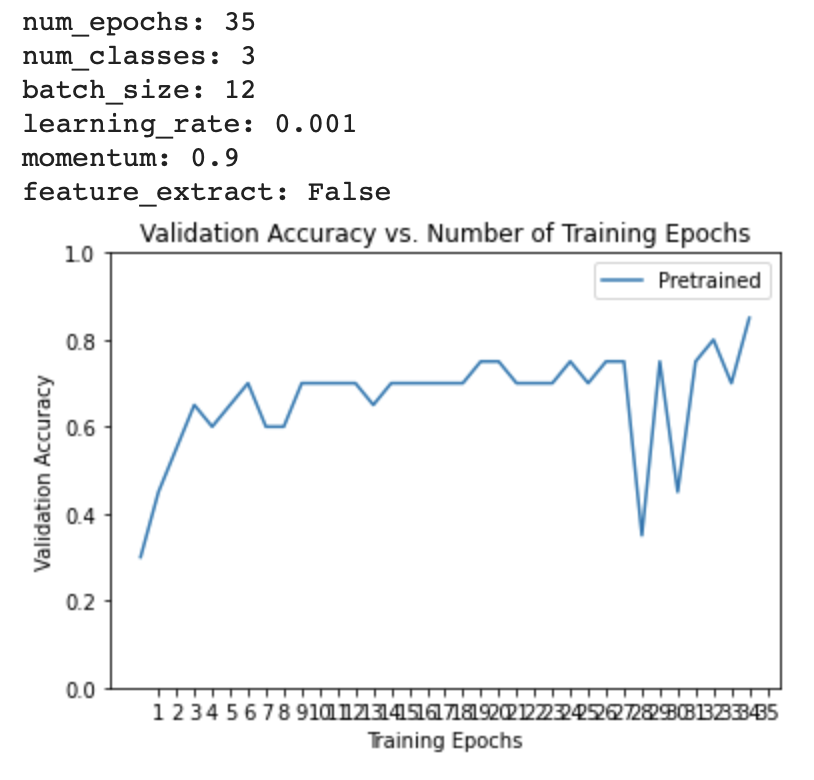
\includegraphics[height=4.166667in, keepaspectratio=true]{./fig/Vision/GoogleColab/Test_Camera_Setup/Resnet18/Screenshot 2020-11-18 at 22.58.45.png}

Tweede test met een aanpassing van de learning rate en een foto van de training set naar test set gebracht

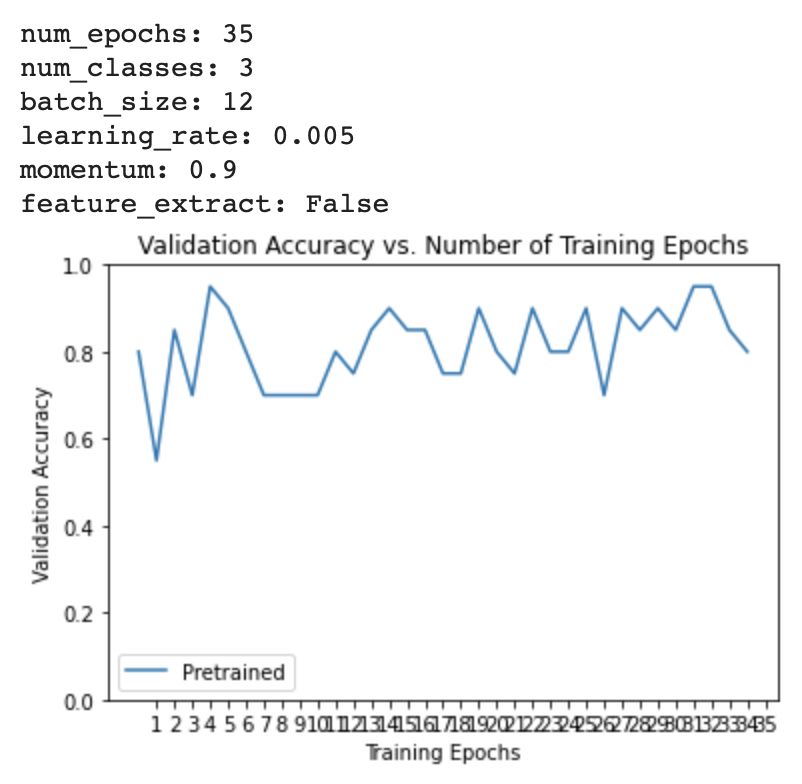
\includegraphics[height=4.166667in, keepaspectratio=true]{./fig/Vision/GoogleColab/Test_Camera_Setup/Resnet18/Screenshot 2020-11-18 at 23.13.23.png}



Next time create results file to get nice overview of all results


